\newpage
\section{脂肪酸甲酯在H-ZSM-5分子筛上的扩散}
\par{目前通过实验测量吸附分子在分子筛中的扩散系数是非常有挑战性的,因为很难将扩散与反应分离,扩散系数只能在相对低温下测量。虽然在任何期望温度下的扩散系数可以在确定指前因子和活化能后根据阿伦尼乌斯方程计算,但从较窄的低温范围得出的这些参数再外推到脂肪酸甲酯催化裂解的高温时可能会产生显著的误差\cite{bu2018diffusion}。}
\par{所以本章使用Materials Studio 8.0软件的Sorption模块和Forcite模块,进行了动力学模拟。主要计算了模型化合物丁酸甲酯在微介孔H-ZSM-5分子筛上的扩散系数。}
\subsection{Sorption 参数设置}\label{Sorption 扩散参数设置}
\par{本节使用Forcite模块与Sorption模块进行动力学模拟,相关参数设置如下:}
\begin{enumerate}
    \item 应用Sorption模块中的固定压力(Fixed Pressure)功能计算在温度673K和压力100kPa下,丁酸甲酯在不同孔径大小的分子筛的饱和吸附量,参数设置和 \ref{Sorption 参数设置} 所设参数一样。这样可以保证是在相同温度和压力下进行的比较。
    \item 应用Sorption模块中的固定吸附量(Fixed Loading)功能和手动放置吸附分子模型到介孔内的方法,分别在H-ZSM-5分子筛中负载对应饱和吸附量的分子个数,其余参数与 \ref{Sorption 参数设置} 相同。
    \item 对负载吸附分子的结构用 Forcite模块进行结构优化(Geometry Optimization)和模拟退火(Anneal),参数设置和 \ref{Forcite 参数设置} 一样。
    \item 然后对负载吸附分子的结构用Forcite 模块的Dynamics功能进行动力学模拟,采用NVT系综,随机给予初始速度,温度选择673K,模拟步长为1fs,模拟步数为100000,总体模拟时间100ps,每5000步输出一次图像用于分析扩散结果。
    \item 将上一步的结果再次进行Forcite Dynamics模拟,采用NVE系综,采用当前速度,模拟步长为1fs,模拟步数为400000,总体模拟时间400ps,每500步输出一次图像用于分析扩散结果。
\end{enumerate}

\subsection{模型验证}
\par{为了验证本文采用的计算扩散系数的方法和参数的正确性,本文将模拟计算出的正己烷分子在不同温度、不同孔径下的H-ZSM-5 分子筛的扩散系数的结果和文献\cite{bu2018diffusion}实验得到的结果相对比,模拟参数按照上文的参数设置。对比结果如\reftab{tab:C6}所示。采用 \ref{分子动力学} 所讲述的斯托克斯 - 爱因斯坦方程计算扩散系数。}
\begin{equation}
    D=\frac{1}{6 N} \lim _{x \rightarrow \infty} \frac{d}{d t} \sum_{i=1}^{N}\left\langle|r(t)-r(0)|^{2}\right\rangle
\end{equation}
\par{式中:$N$表示吸附分子总的数量;$r(0)$表示吸附分子质心的初始位置坐标;$r(t)$表示吸附分子在时间$t$时的质心坐标;$\left\langle|r(t)-r(0)|^{2}\right\rangle$表示扩散分子均方位移(MSD)的系综平均。}
\par{吸附分子在扩散过程中的均方位移可以直接从Materials Studio 8.0软件分析得出。以正己烷在60Å介孔H-ZSM-5分子筛的扩散为例,其均方位移随时间的变化曲线如\reffig{fig:C6}所示。}
\begin{figure}[H]
    \centering
        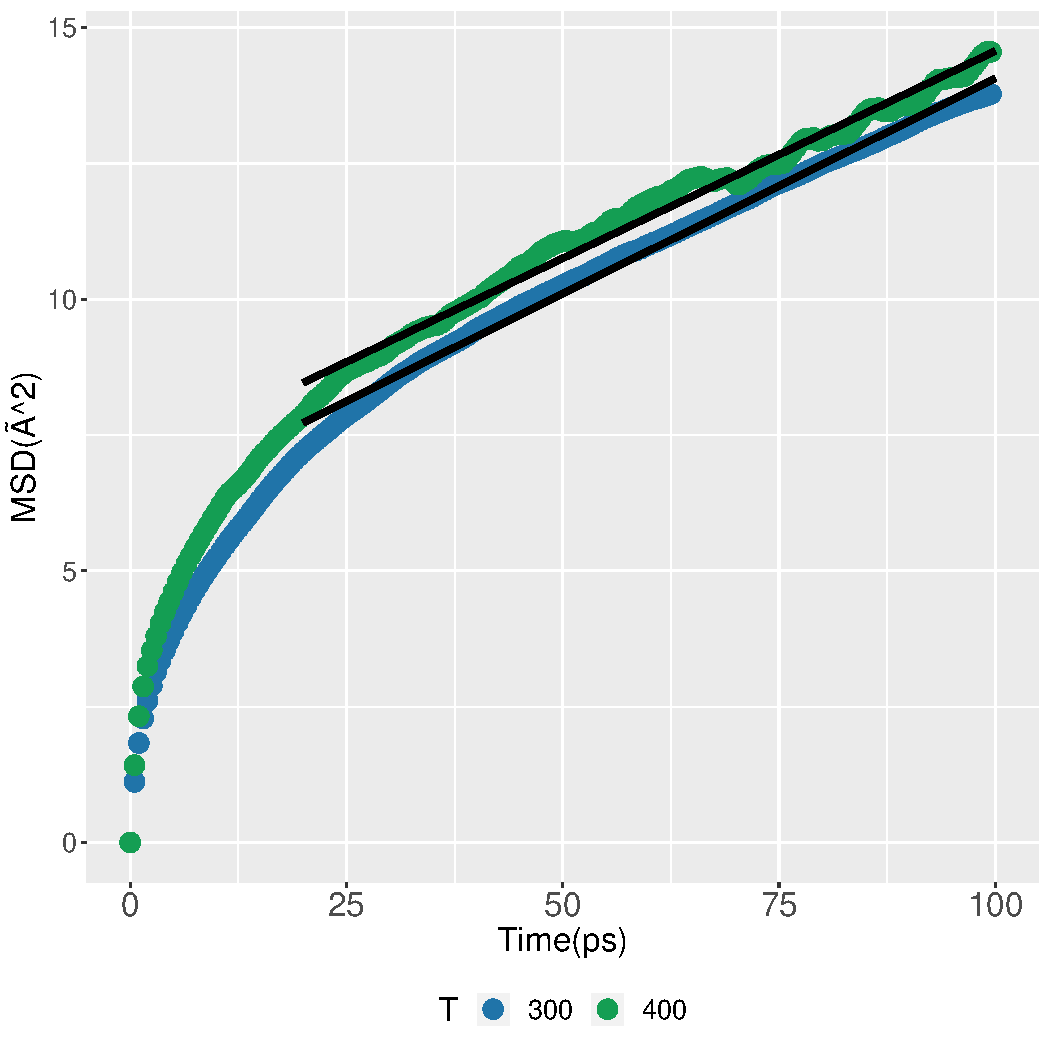
\includegraphics[width=0.5\linewidth]{figure/Diffusion/C6.pdf}
    \caption{正己烷均方位移随时间变化曲线图}
    \label{fig:C6}
\end{figure}
\par{从\reffig{fig:C6}中看出,MSD曲线大致为线性,曲线刚开始为对数形式,后半部分为直线,符合 \ref{分子动力学} 中文献所描述的MSD曲线的特点。所以根据斯托克斯 - 爱因斯坦方程拟合计算直线部分的斜率,得到各个条件下的扩散系数,并与文献结果相对比,具体数值见\reftab{tab:C6}。}
\begin{table}[H]
	\small
	\centering
	\caption{正己烷扩散系数模拟与实验数据对比表}
	\begin{tabular}{p{2.5cm}<{\centering}p{2cm}<{\centering}p{3cm}<{\centering}P{2.2}P{2.5}}
        \toprule
        孔径&\makecell{温度\\(K)}&\makecell{MSD曲线斜率\\(Å$^2$/ps)}&\multicolumn{1}{p{3cm}<{\centering}}{\makecell{计算扩散系数\\(×$10^{-10}$m$^2$/s)}}&\multicolumn{1}{p{3cm}<{\centering}}{\makecell{实验扩散系数\\(×$10^{-10}$m$^2$/s)}}\\
        \midrule
        \multirow{2}{*}{60Å介孔}&300&0.0795&13.25&12.4±0.5\\
        &400&0.0909&15.15&18.3±2.5\\
        \hline
        20Å介孔&300&0.0069&1.15&1.4±0.3\\
		\bottomrule
	\end{tabular}
	\label{tab:C6}
\end{table}
\par{由\reftab{tab:C6}可知,计算得到的结果和实验结果非常吻合,均处在误差范围内,所以本文采取的模型结构和力场是合理的。下面验证动力学模拟的参数设置是否合理。}
\par{本文对扩散模型进行了两次Forcite Dynamics模拟,首先在NVT系综模拟以确保系统温度达到平衡,在此基础下进行的NVE系综模拟时,体系温度会维持在一个相对恒定的水平。\reffig{fig:Temperature}为300k下正己烷在NVE系综扩散模拟中体系温度随着时间的变化。由图可知,己烷分子在整个动力学模拟过程中体系温度均处于较为恒定(300k)的状态,虽然有波动,但相对误差并未超过5\%,总体处于一个稳定范围。因此在模拟过程中,体系处在动力学平衡状态。}
\begin{figure}[H]
    \centering
        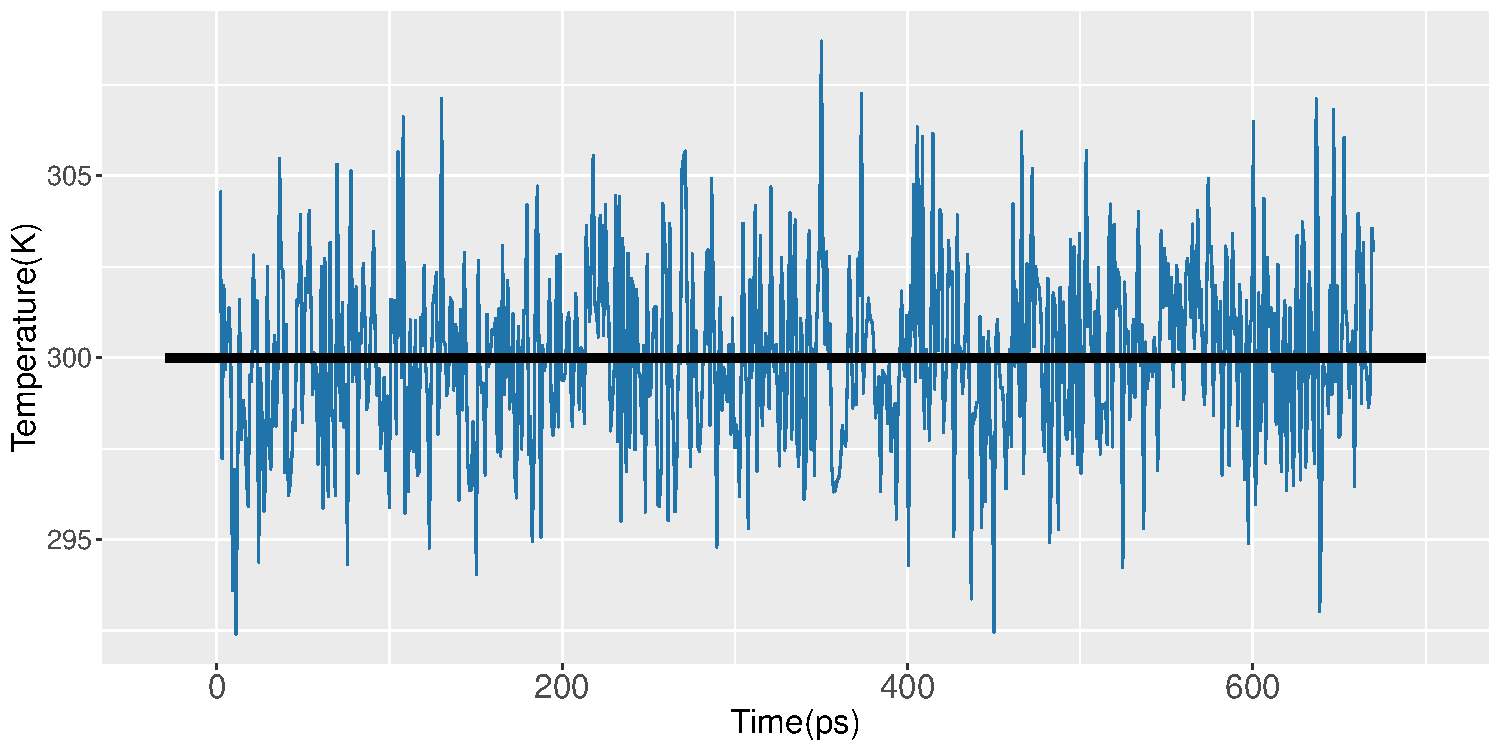
\includegraphics[height=0.5\textwidth]{figure/Diffusion/Temperature.pdf}
    \caption{正己烷分子在动力学模拟时的温度随时间变化图}
    \label{fig:Temperature}
\end{figure}
\subsection{模拟结果}
\par{本节主要分析了丁酸甲酯在不同孔径的分子筛内的扩散情况,包括了丁酸甲酯在介孔内的扩散、从介孔到微孔的扩散,在微孔内的扩散。}

\subsubsection{丁酸甲酯在介孔内的扩散}
\par{本小节主要讨论了丁酸甲酯在微孔和介孔中的扩散情况,说明了介孔对吸附分子扩散系数的影响。}
\par{首先先将丁酸甲酯放置在微孔和介孔中:用固定吸附并结构优化的方式将丁酸甲酯放置到微孔中;用手动放置并结构优化的方式将丁酸甲酯放置到介孔中。放置的分子个数由在673K、100kPa参数条件下的固定压力功能算出,分别为63、42和90个。以分子筛的C方向为例,如\reffig{fig:MMM}所示。}

\begin{figure}[H]
    \centering

    \subfigure[微孔]{
    \begin{minipage}[t]{0.3333\linewidth}
    \centering
    \includegraphics[width=2in]{figure/Diffusion/1MM.png}
    %\caption{fig1}
    \end{minipage}%
    }%
    \subfigure[20Å介孔]{
    \begin{minipage}[t]{0.3333\linewidth}
    \centering
    \includegraphics[width=2in]{figure/Diffusion/1M20.png}
    %\caption{fig2}
    \end{minipage}%
    }%
    \subfigure[60Å介孔]{
    \begin{minipage}[t]{0.3333\linewidth}
    \centering
    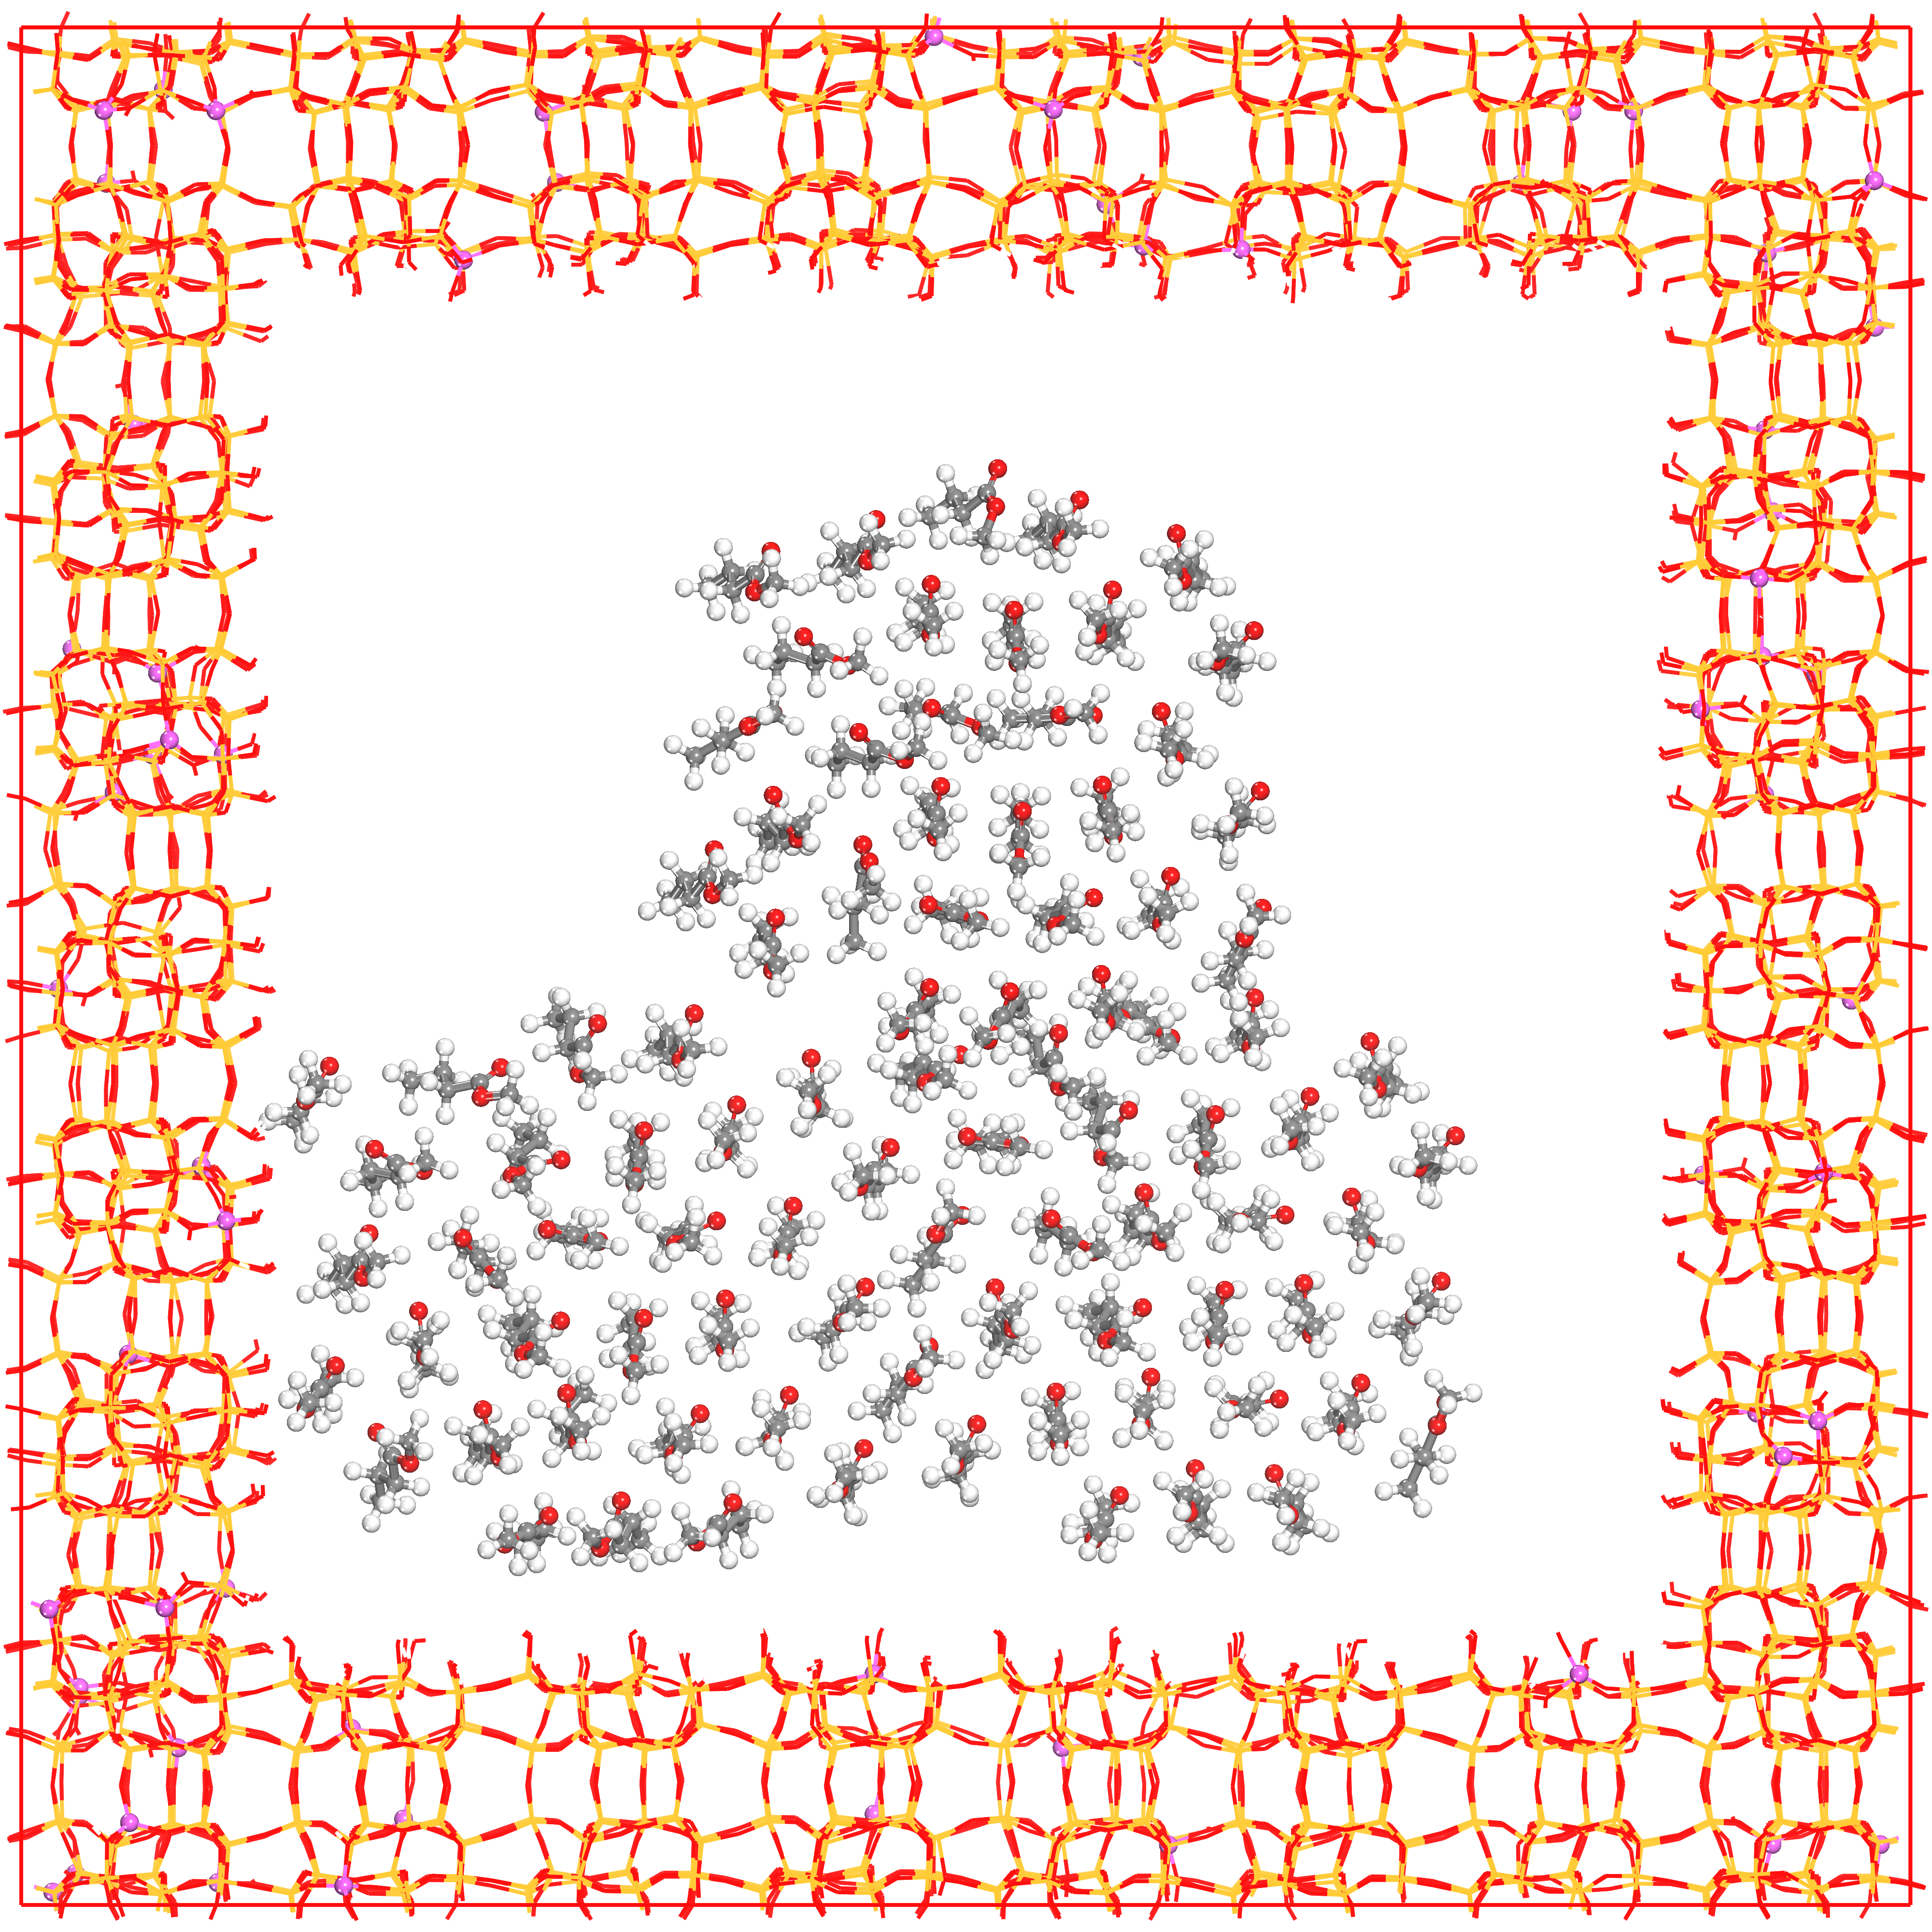
\includegraphics[width=2in]{figure/Diffusion/1M60.png}
    %\caption{fig2}
    \end{minipage}%
    }%
    \caption{丁酸甲酯在微孔和介孔内动力学模拟的初始位置示意图}
    \label{fig:MMM}
\end{figure}

\par{然后采用Forcite模块先后进行NVT和NVE系综的动力学模拟,设置参数如 \ref{Sorption 扩散参数设置} 所示,得到了丁酸甲酯在微介孔的均方位移随时间的变化曲线,如\reffig{fig:MSDd}所示。}
\begin{figure}[H]
    \centering

    \subfigure[微孔]{
    \begin{minipage}[t]{0.3333\linewidth}
    \centering
    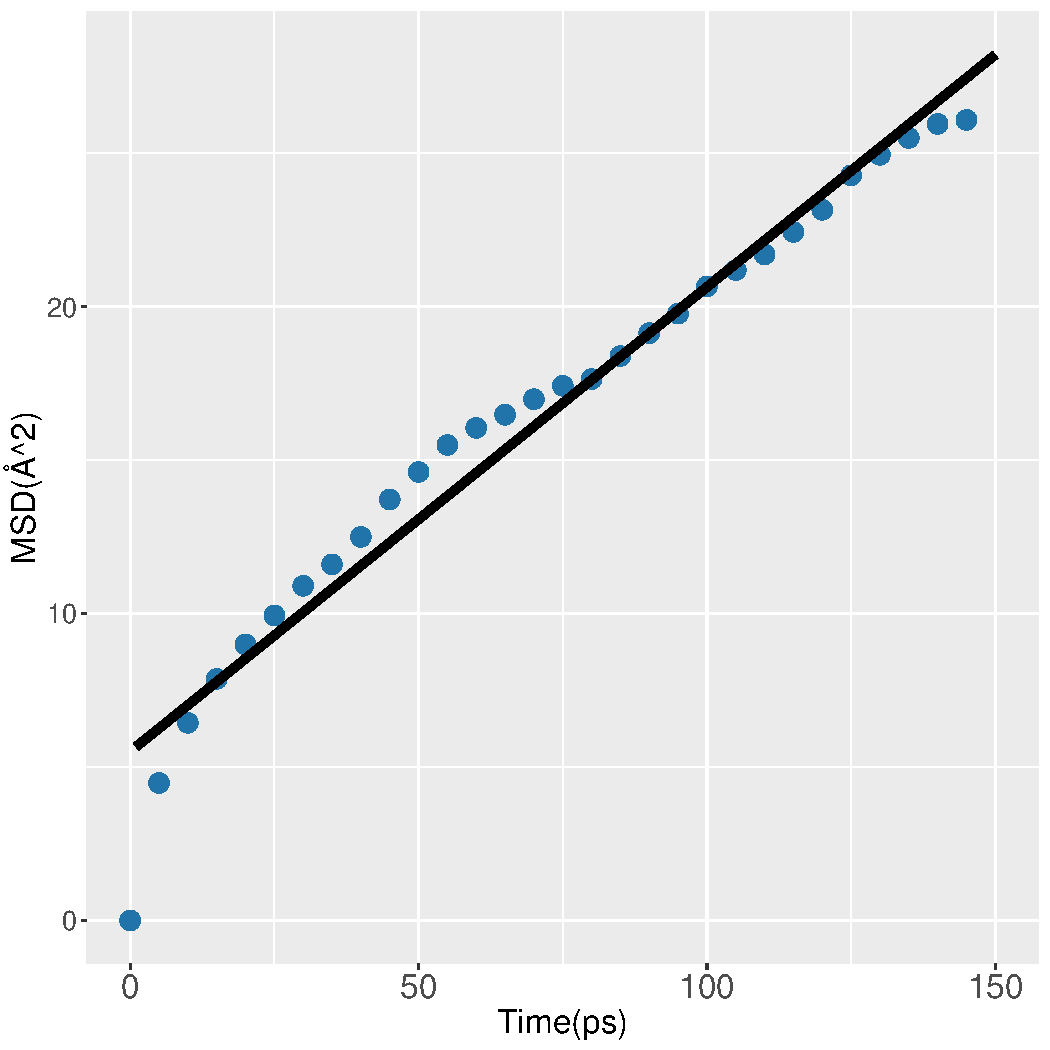
\includegraphics[width=2in]{figure/Diffusion/MSDMM.pdf}
    \end{minipage}%
    }%
    \subfigure[20Å介孔]{
    \begin{minipage}[t]{0.3333\linewidth}
    \centering
    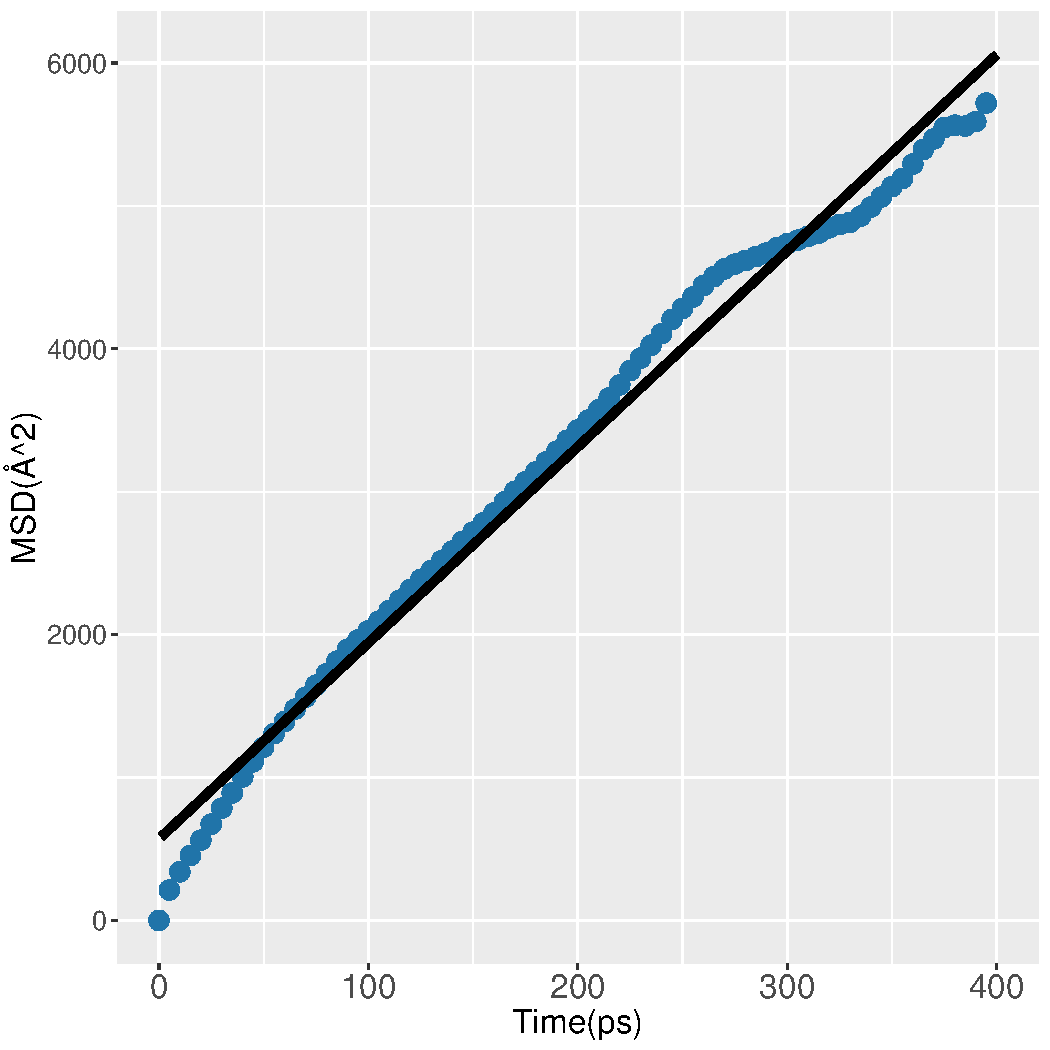
\includegraphics[width=2in]{figure/Diffusion/MSDM20.pdf}
    %\caption{fig2}
    \end{minipage}%
    }%
    \subfigure[60Å介孔]{
    \begin{minipage}[t]{0.3333\linewidth}
    \centering
    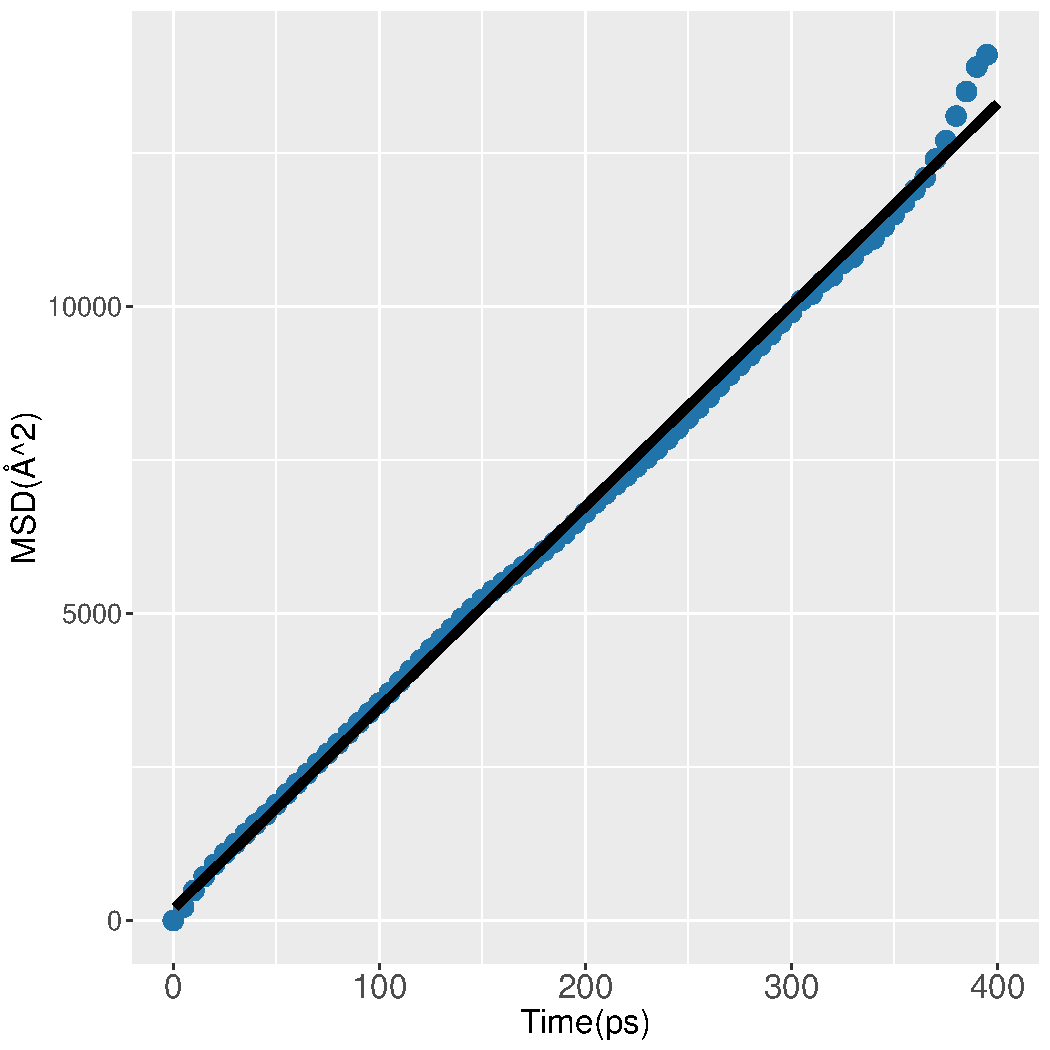
\includegraphics[width=2in]{figure/Diffusion/MSDM60.pdf}
    %\caption{fig2}
    \end{minipage}%
    }%
    \caption{丁酸甲酯在不同孔径H-ZSM-5分子筛的MSD vs. Time图}
    \label{fig:MSDd}
\end{figure}
\par{从\reffig{fig:MSDd}中看出,丁酸甲酯在不同孔径下的MSD曲线大致为线性,满足斯托克斯 - 爱因斯坦方程。根据 \ref{分子动力学} 中斯托克斯 - 爱因斯坦方程计算出在微介孔的扩散系数,具体数值见\reftab{tab:MSD}。}

\begin{table}[H]
	\small
	\centering
	\caption{丁酸甲酯在不同孔径H-ZSM-5分子筛中的扩散系数对比表}
	\begin{tabular}{p{2.5cm}<{\centering}P{2.4}P{3.4}p{2.5cm}<{\centering}P{4.2}}
        \toprule
        孔径&\multicolumn{1}{p{2.5cm}<{\centering}}{\makecell{斜率\\(Å$^2$/ps)}}&\multicolumn{1}{p{2.5cm}<{\centering}}{\makecell{截距\\(Å$^2$)}}&R$^2$&\multicolumn{1}{p{4cm}<{\centering}}{\makecell{扩散系数\\(×$10^{-10}$m$^2$/s)}}\\
        \midrule
        微孔&0.1514&5.5047&0.9613&25.23\\
        介孔20Å&13.7192&57.0054&0.9855&2286.53\\
        介孔60Å&32.7761&187.6688&0.9967&5462.68\\
        \bottomrule
	\end{tabular}
	\label{tab:MSD}
\end{table}
\par{由\reftab{tab:MSD}可知在催化裂化反应条件下,模型化合物丁酸甲酯在不同孔径的H-ZSM-5分子筛中的扩散能力为60Å介孔> 20Å介孔$\gg$微孔的扩散速率。与微孔H-ZSM-5 相比,在20Å 介孔中测量的扩散系数增加了2个数量级。然而,增加介孔H-ZSM-5 的孔径对扩散的影响不大,随着孔径从20Å增加到60Å,计算得到的扩散系数仅增加1.4倍。}

\subsubsection{丁酸甲酯从介孔到微孔的扩散}
\par{本小节主要讨论了丁酸甲酯从介孔孔道到微孔孔道的情况。}
\par{微孔分子筛的孔径大小通过其限制作用,基本上可以影响吸附分子的扩散,从而影响吸附分子的取向。比如Bu\cite{bu2016diffusion}证明了对二甲苯分子主要是平行于直孔道扩散的,因为其最长主轴的长度(9.1Å)大于微孔H-ZSM-5分子筛相对较小的孔径。而本文的丁酸甲酯的最长主轴的长度(7.8Å)也大于H-ZSM-5分子筛的孔径大小,所以丁酸甲酯必须以一定的取向才能进入微孔,否则将会被分子筛弹开。以60Å介孔为例,以一帧5ps的速度,\reffig{fig:MSDa}展示了扩散刚开始的35ps这段时间内丁酸甲酯的运动轨迹。}
\begin{figure}[H]
    \centering

    \subfigure[0ps]{
    \begin{minipage}[t]{0.25\linewidth}
    \centering
    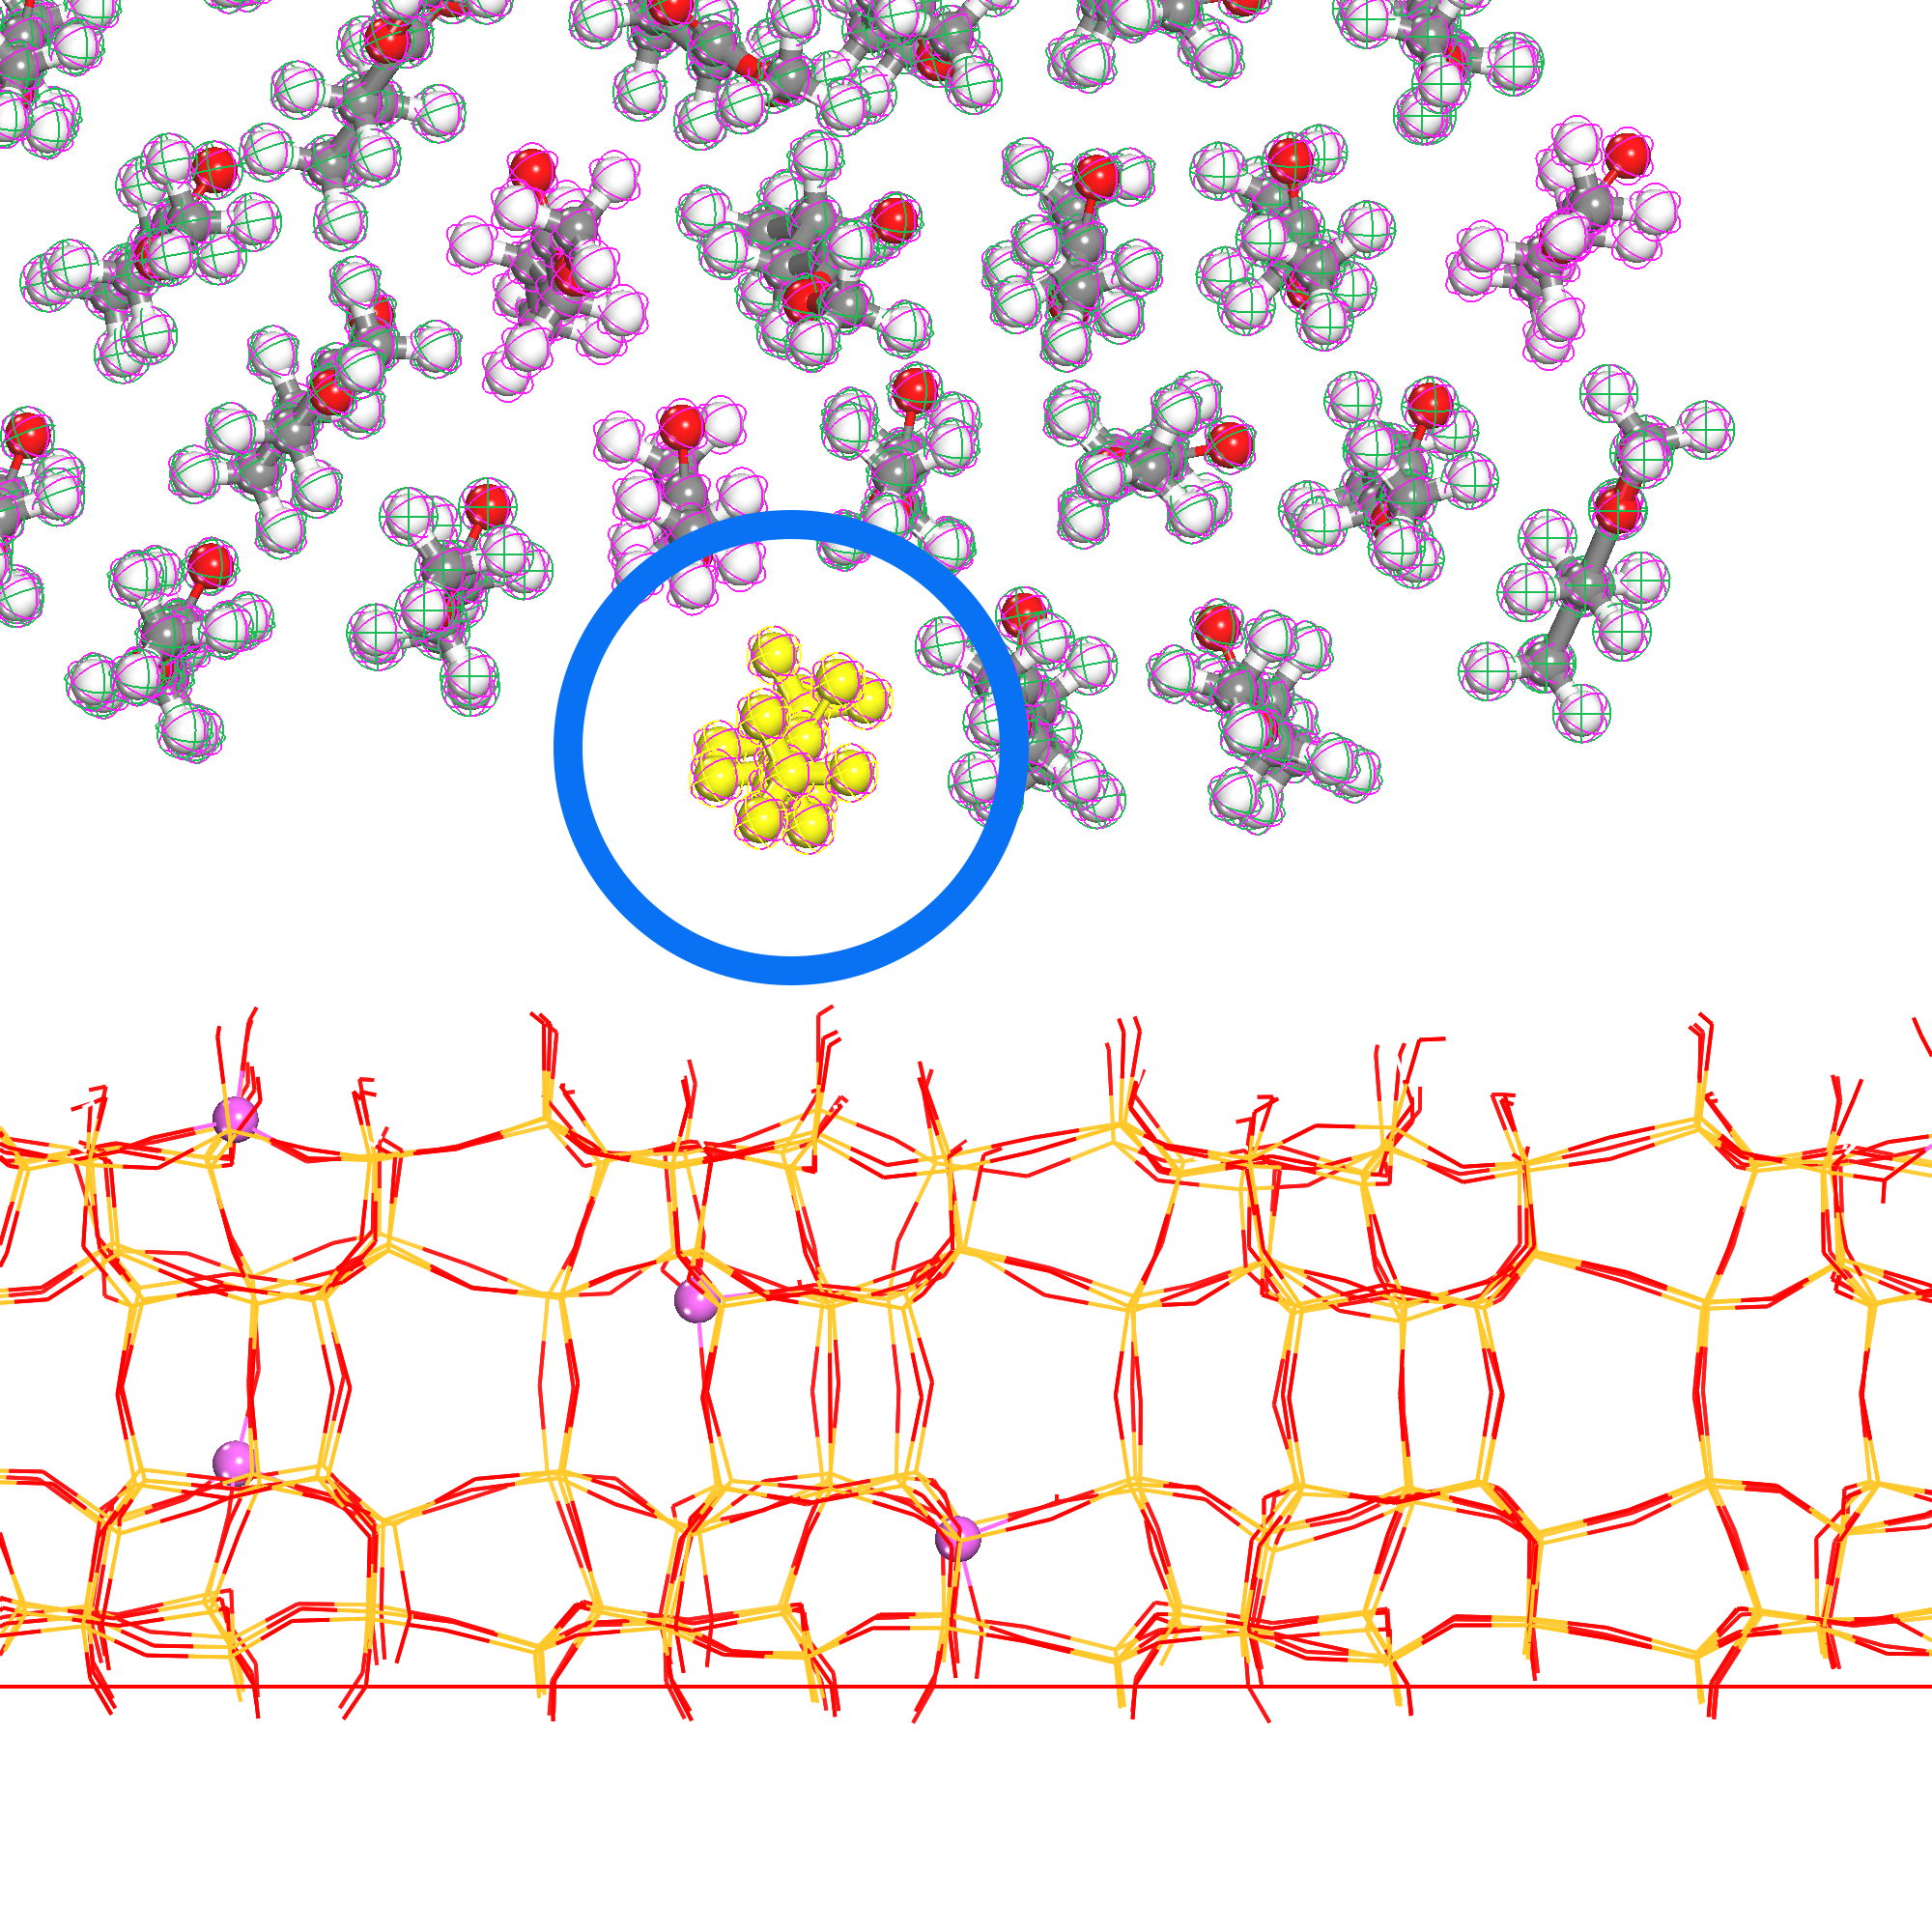
\includegraphics[width=1.35in]{figure/Diffusion/1.png}
    \end{minipage}%
    }%
    \subfigure[5ps]{
    \begin{minipage}[t]{0.25\linewidth}
    \centering
    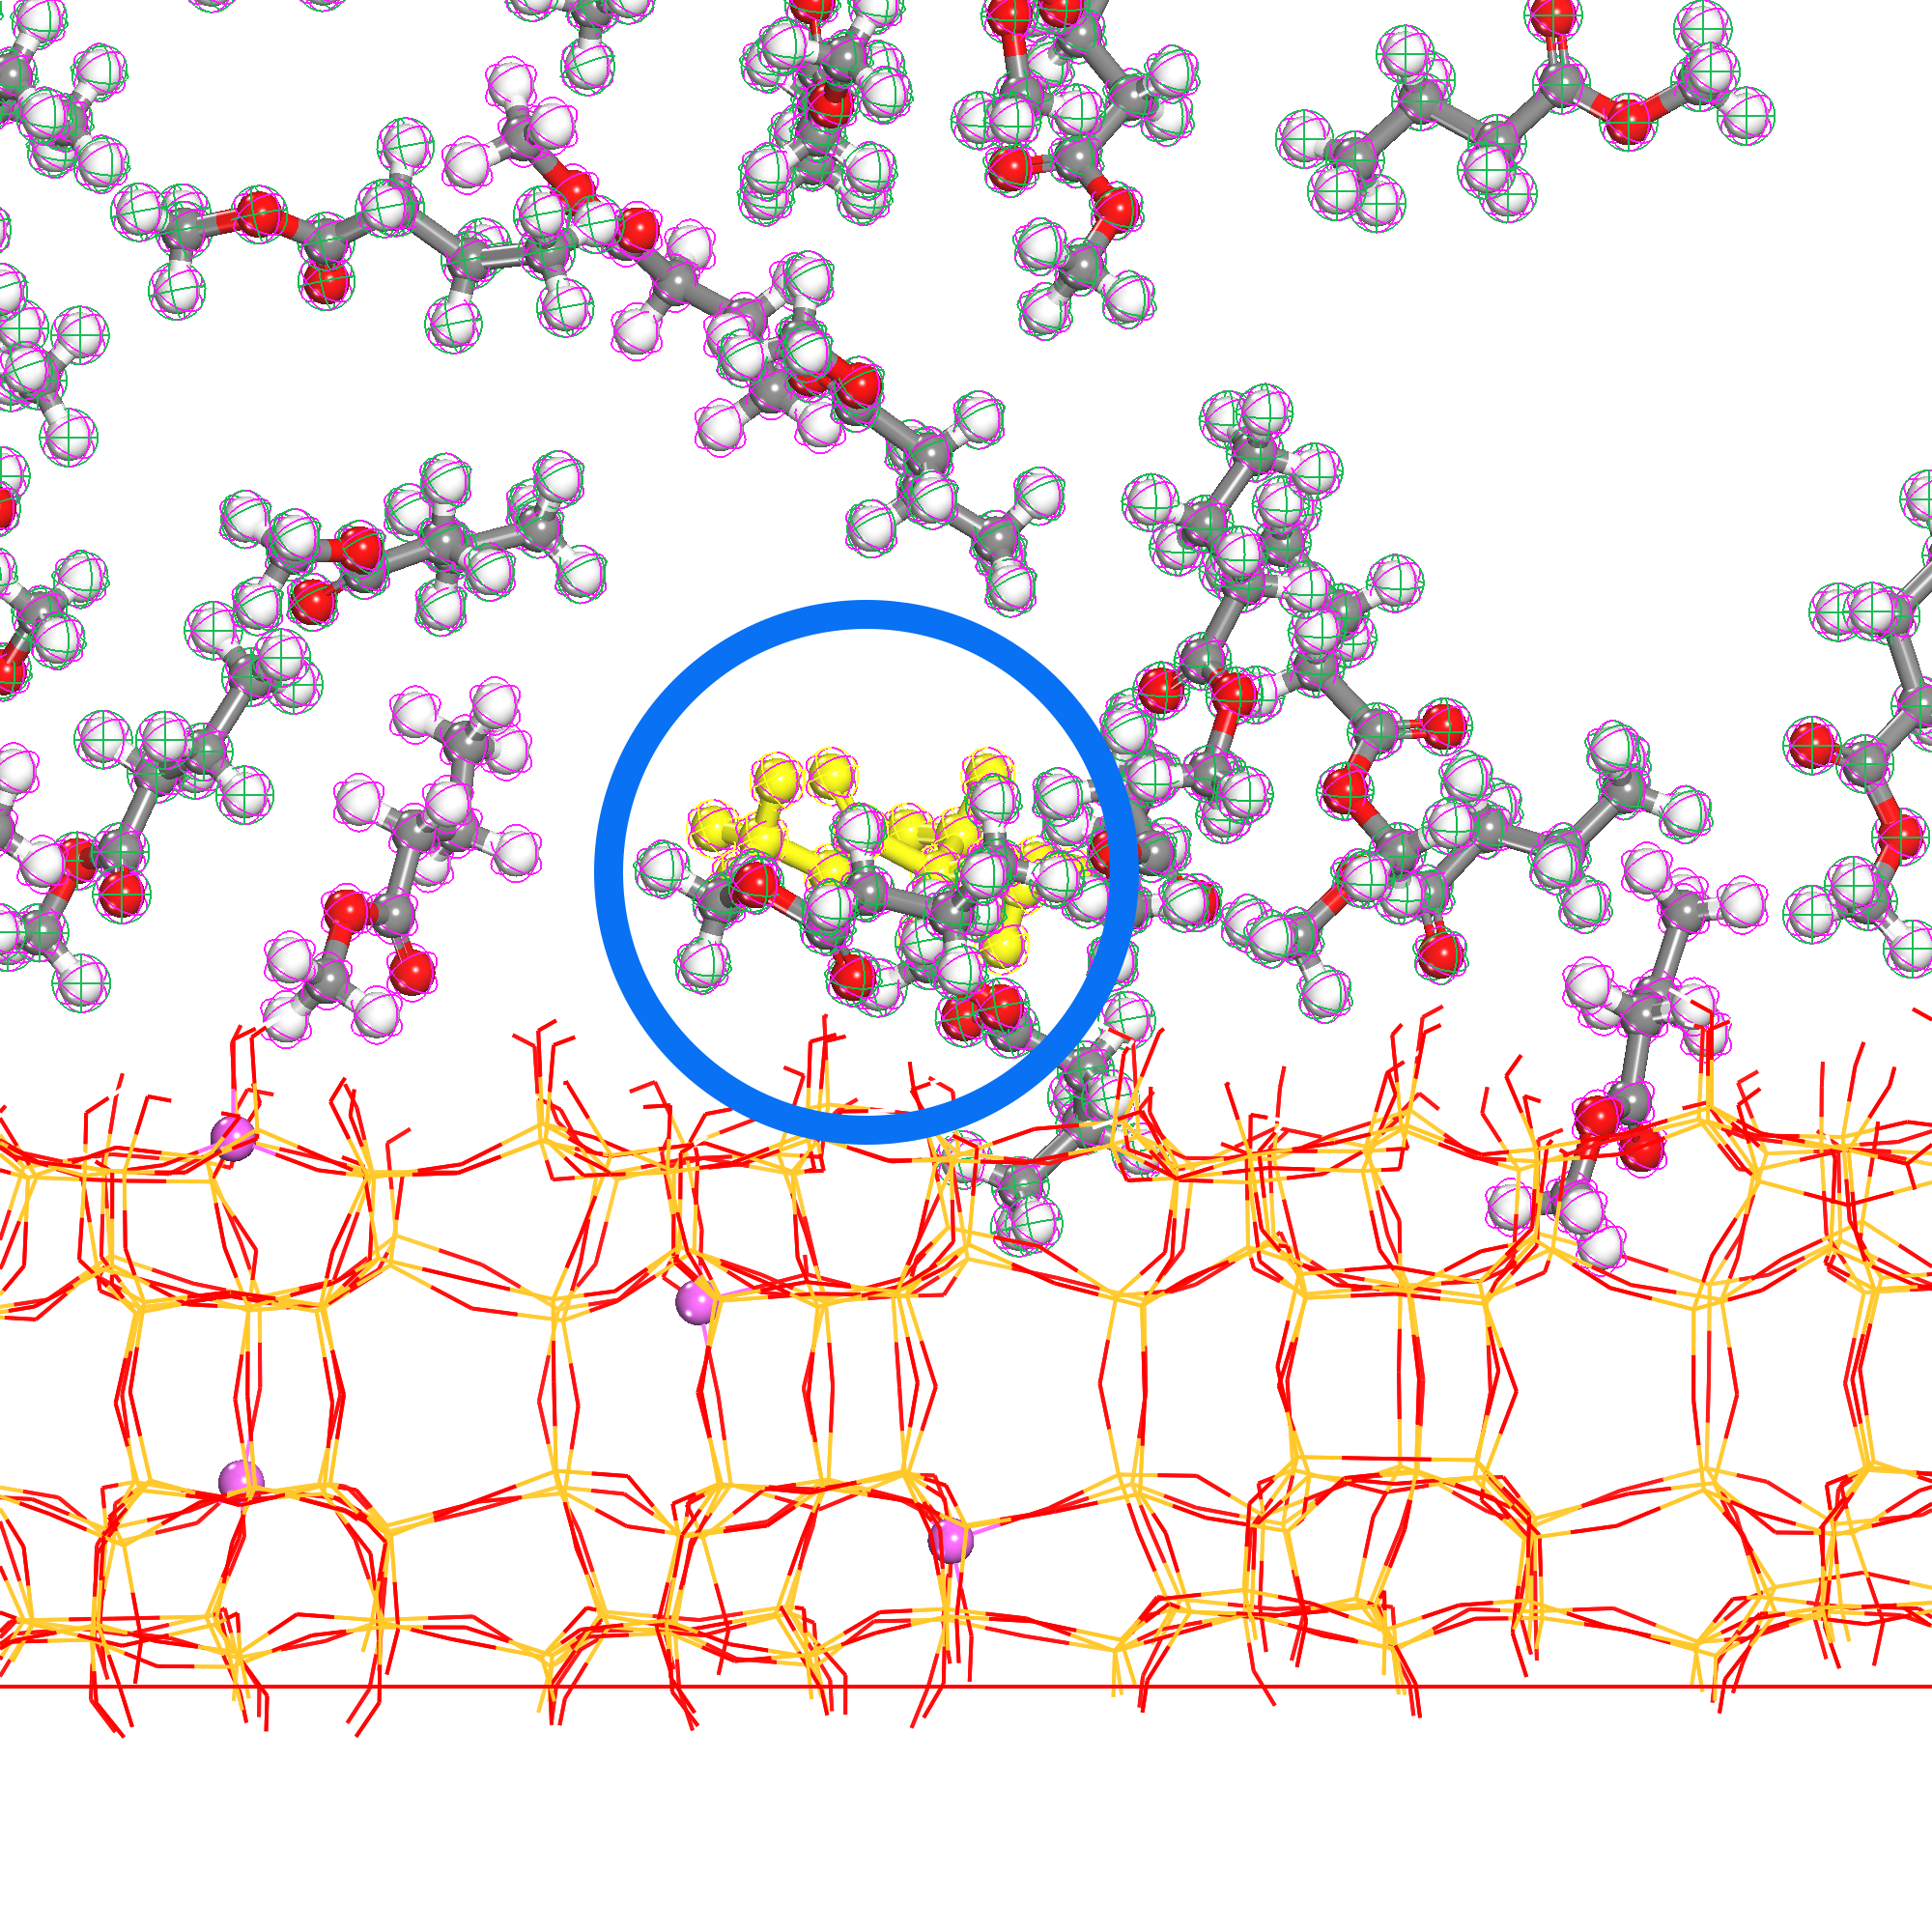
\includegraphics[width=1.35in]{figure/Diffusion/2.png}
    %\caption{fig2}
    \end{minipage}%
    }%
    \subfigure[10ps]{
    \begin{minipage}[t]{0.25\linewidth}
    \centering
    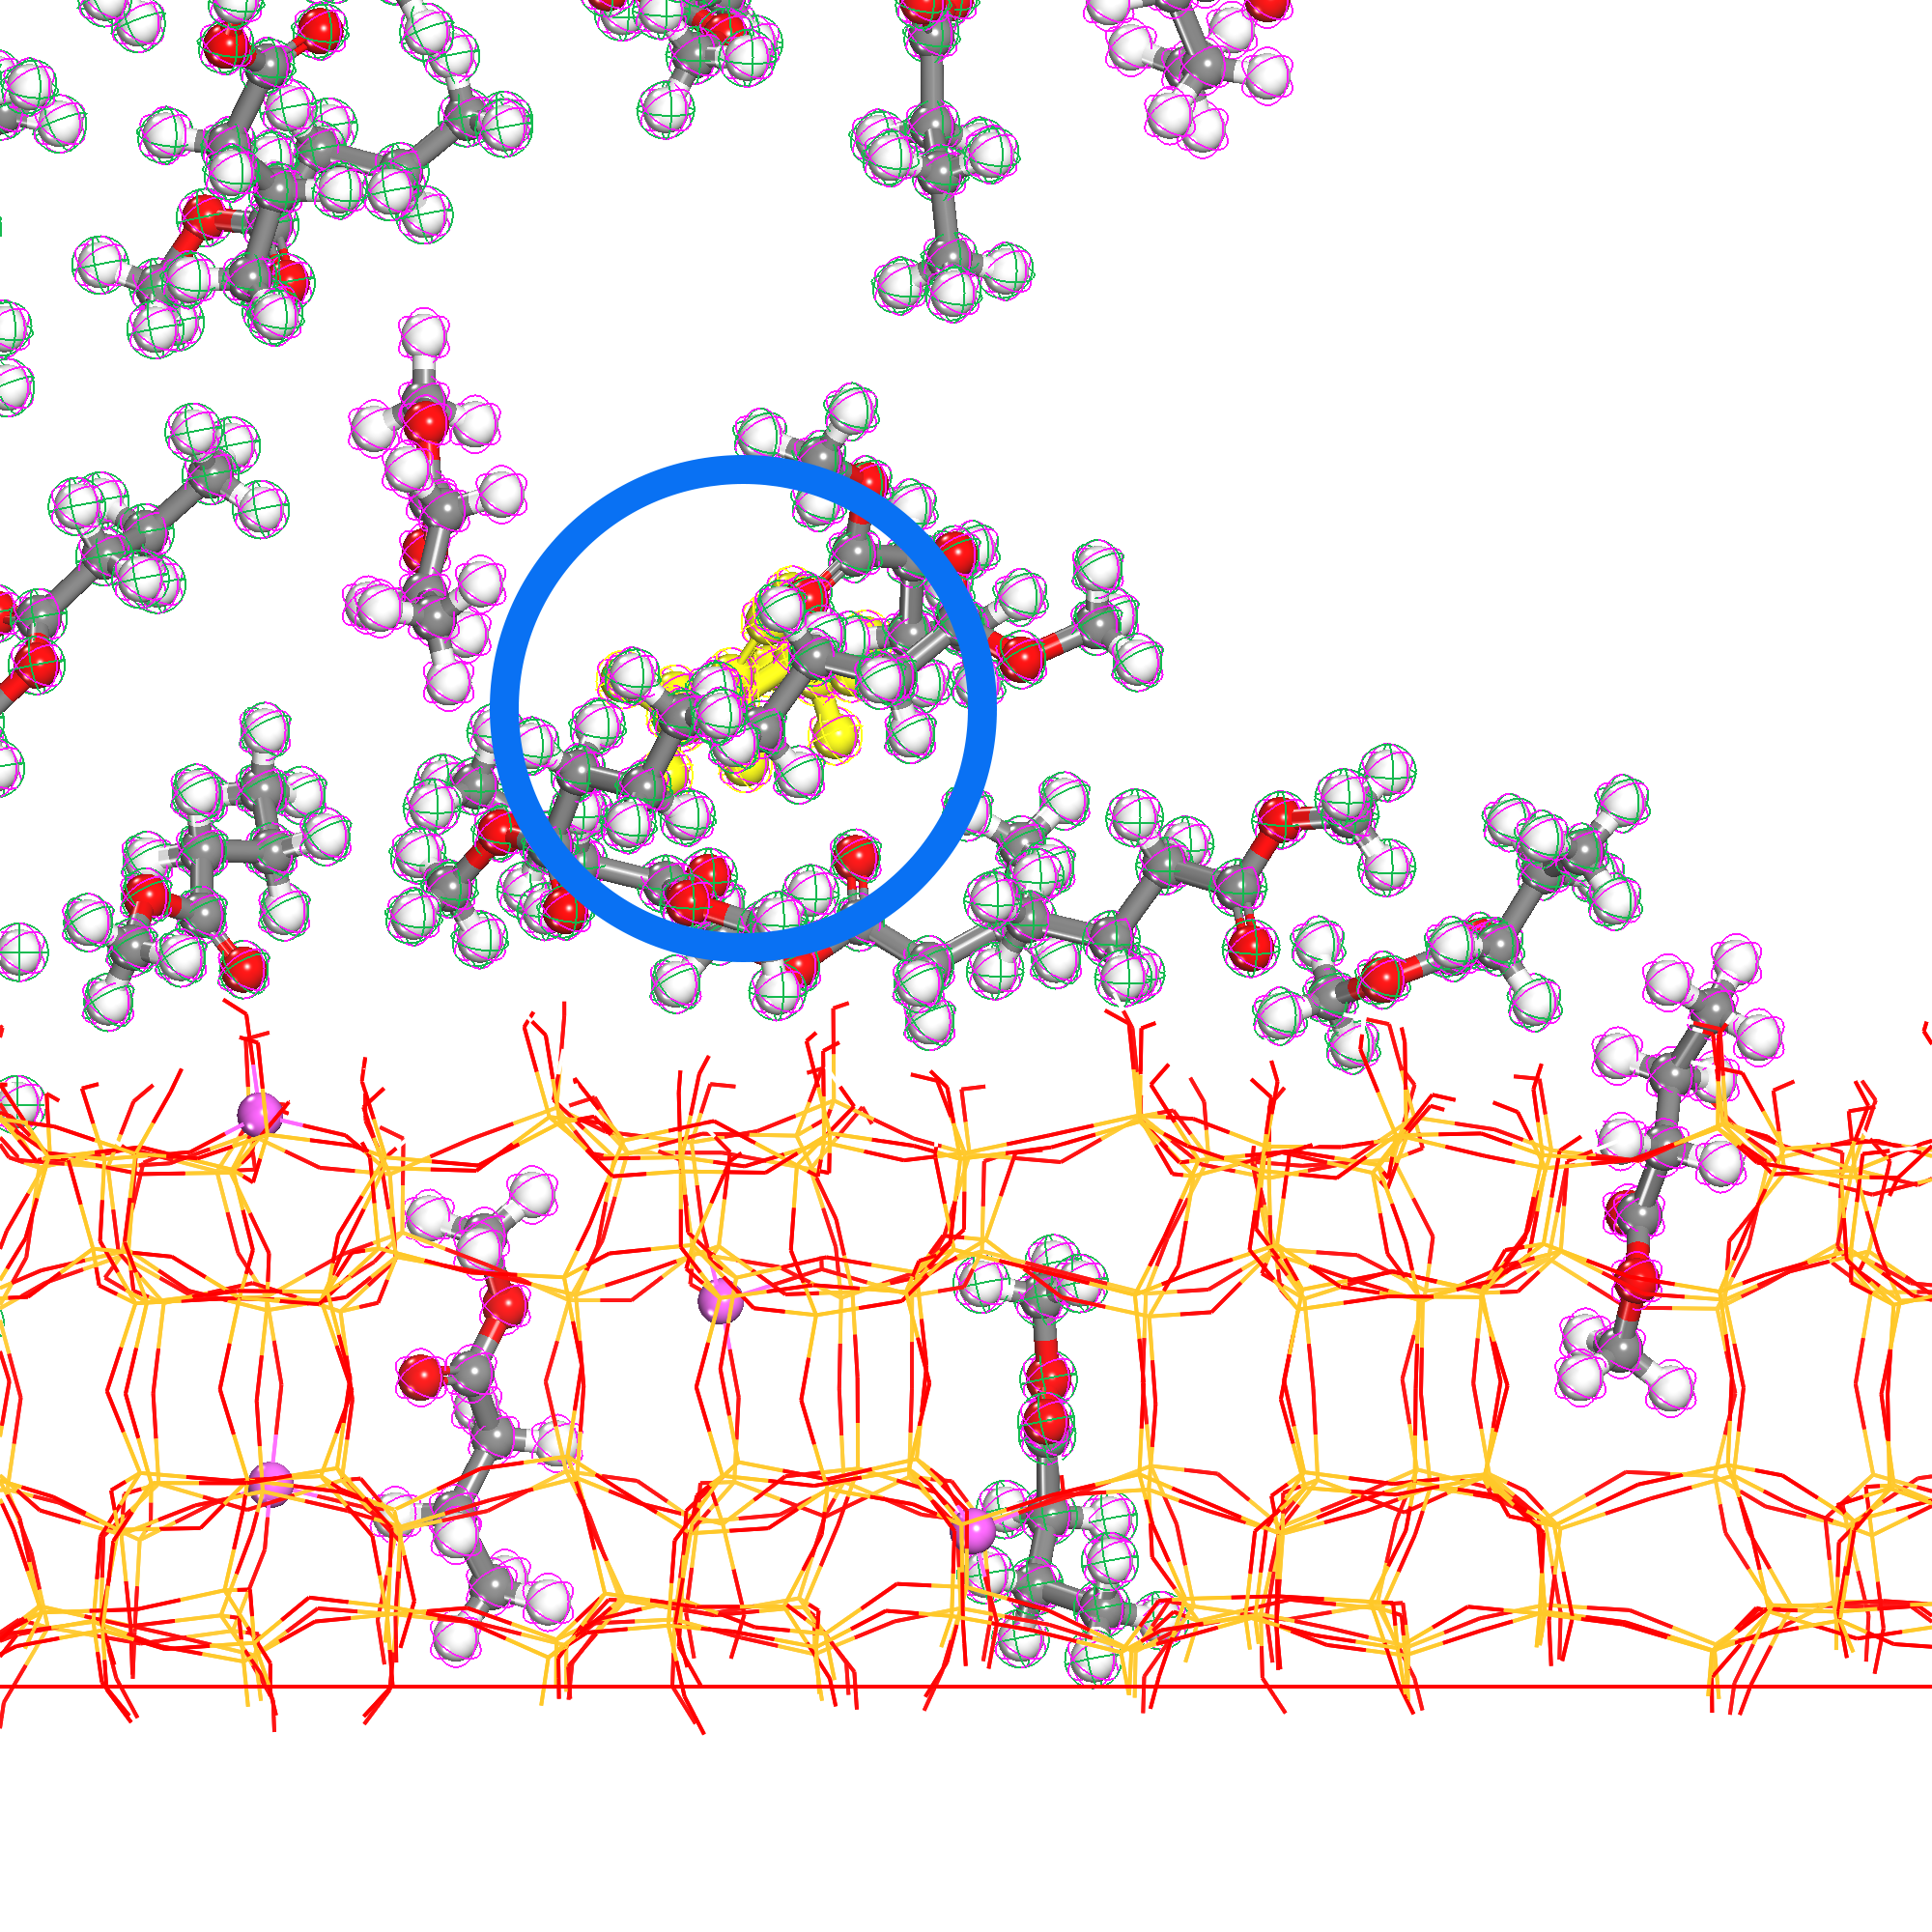
\includegraphics[width=1.35in]{figure/Diffusion/3.png}
    %\caption{fig2}
    \end{minipage}%
    }%
    \subfigure[15ps]{
    \begin{minipage}[t]{0.25\linewidth}
    \centering
    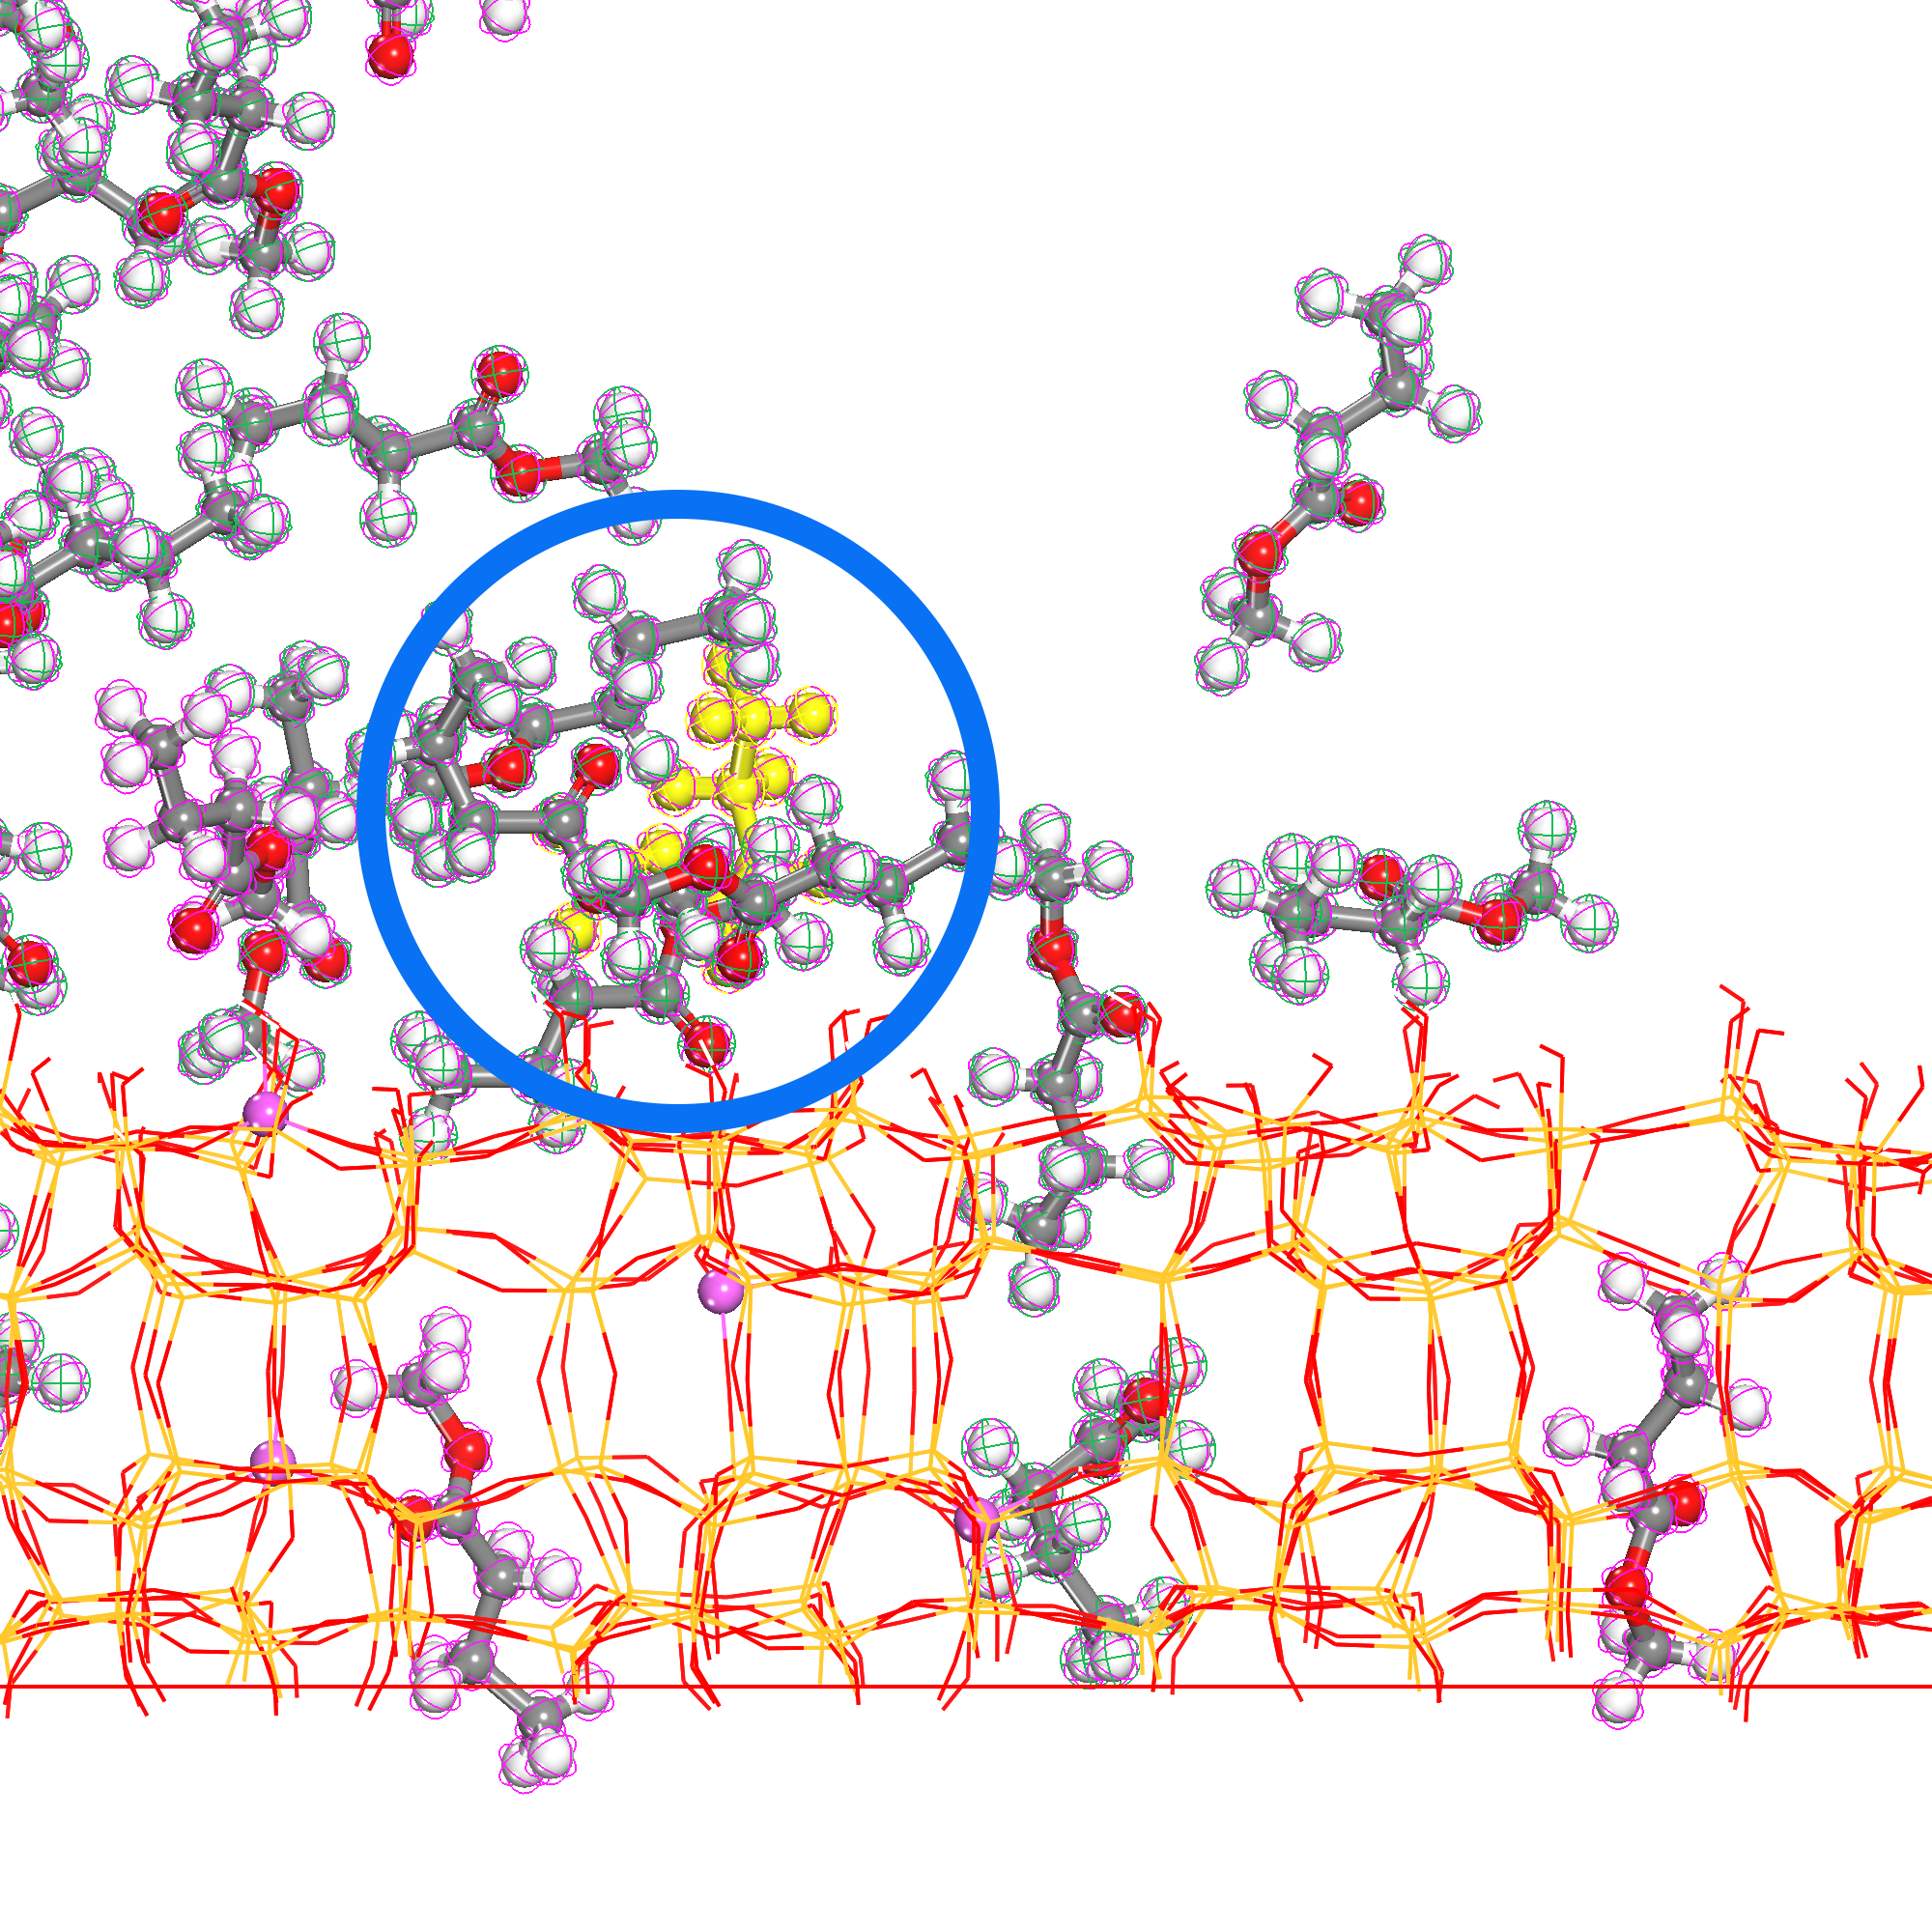
\includegraphics[width=1.35in]{figure/Diffusion/4.png}
    \end{minipage}%
    }%

    \subfigure[20ps]{
    \begin{minipage}[t]{0.25\linewidth}
    \centering
    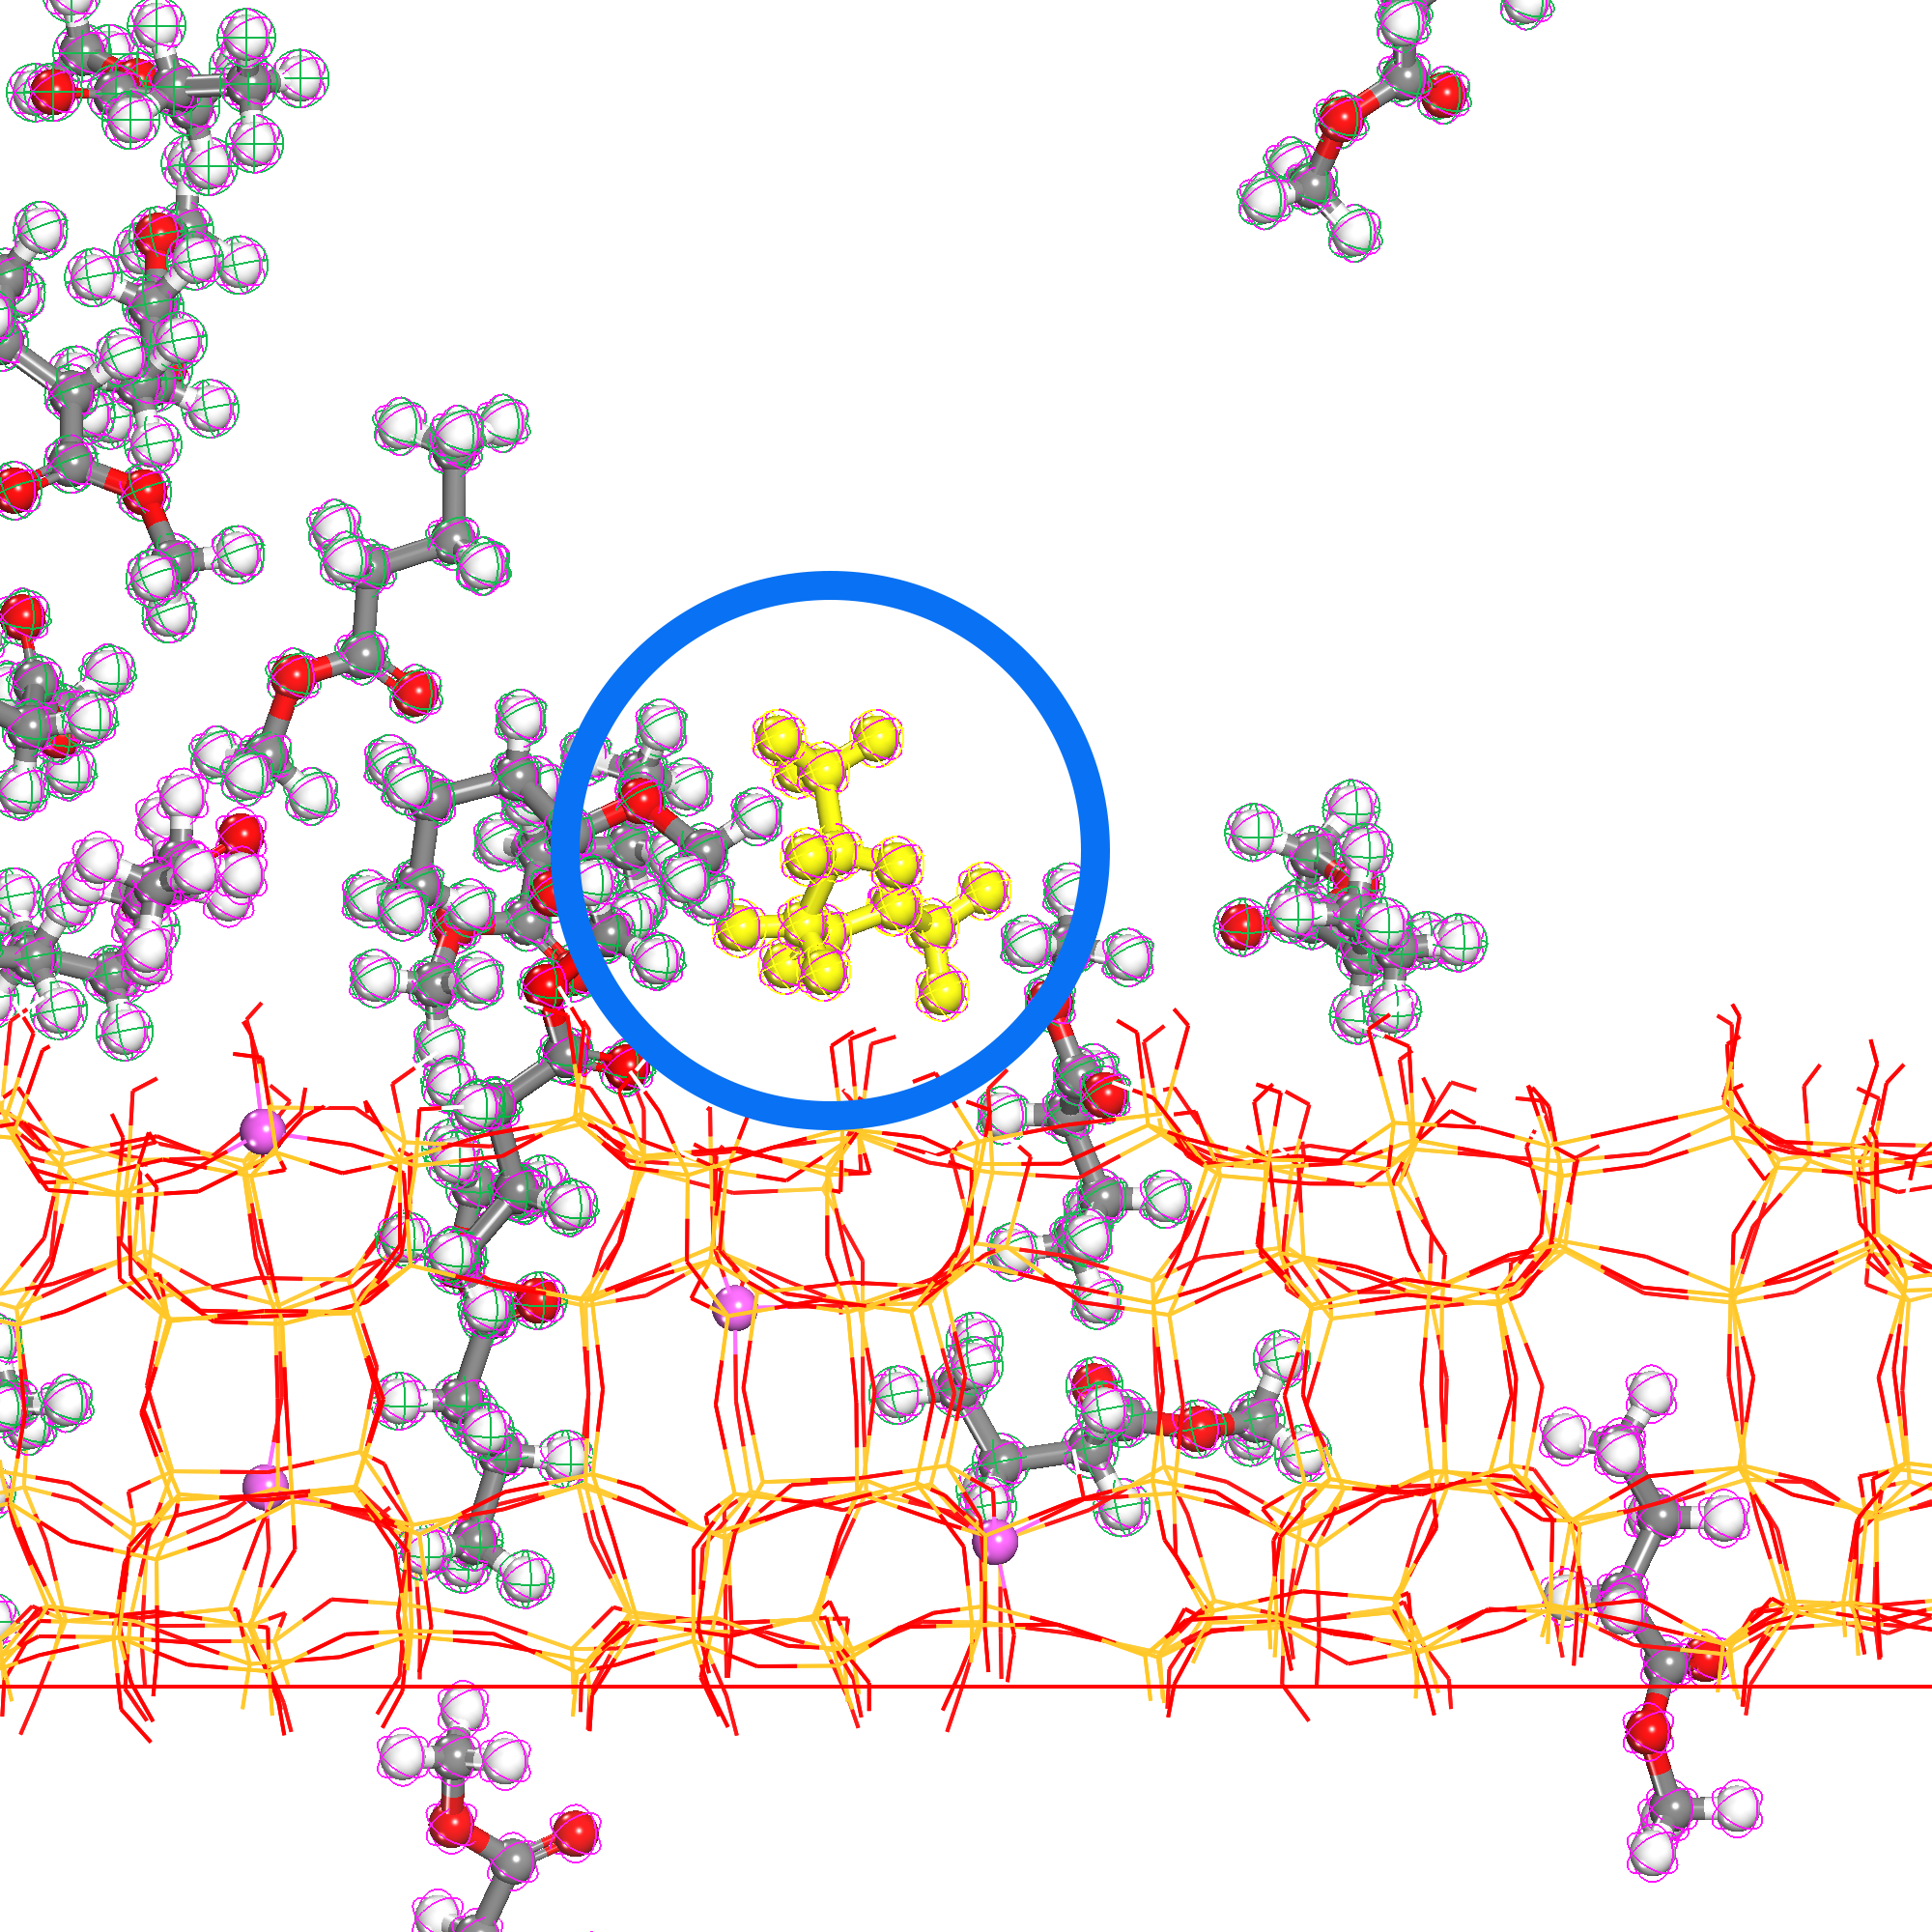
\includegraphics[width=1.35in]{figure/Diffusion/5.png}
    %\caption{fig2}
    \end{minipage}%
    }%
    \subfigure[25ps]{
    \begin{minipage}[t]{0.25\linewidth}
    \centering
    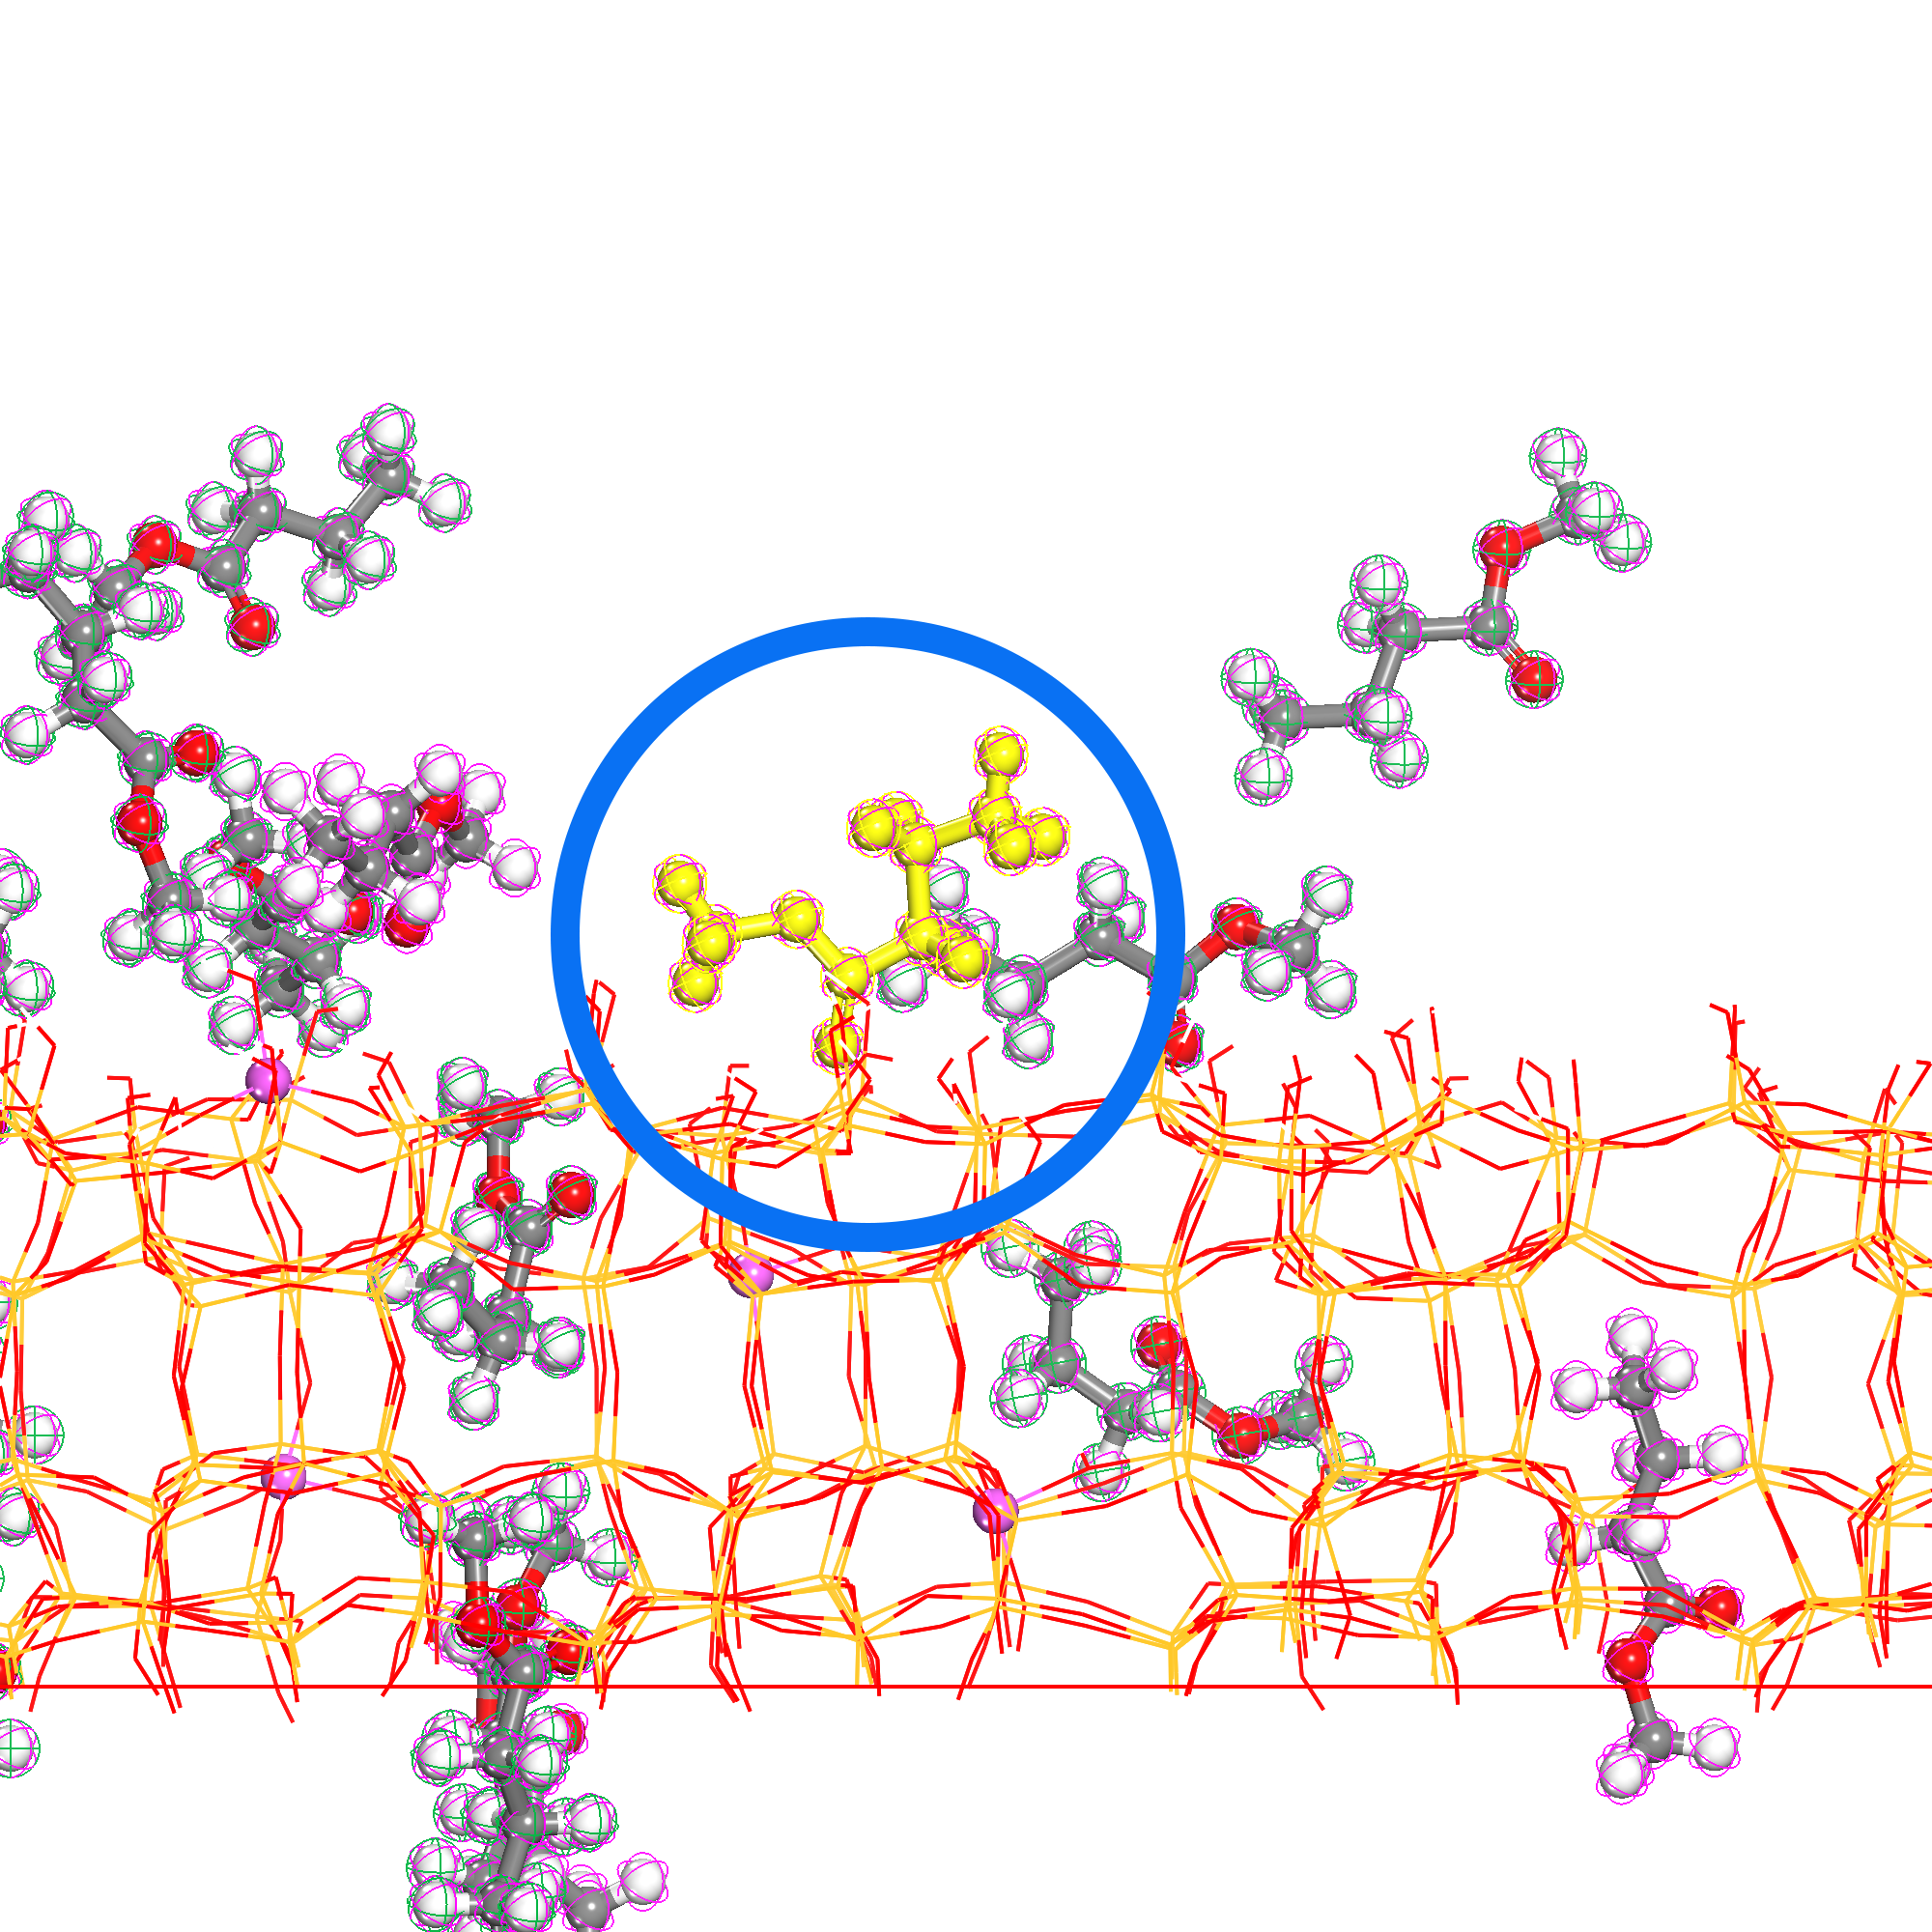
\includegraphics[width=1.35in]{figure/Diffusion/6.png}
    %\caption{fig2}
    \end{minipage}%
    }%
    \subfigure[30ps]{
    \begin{minipage}[t]{0.25\linewidth}
    \centering
    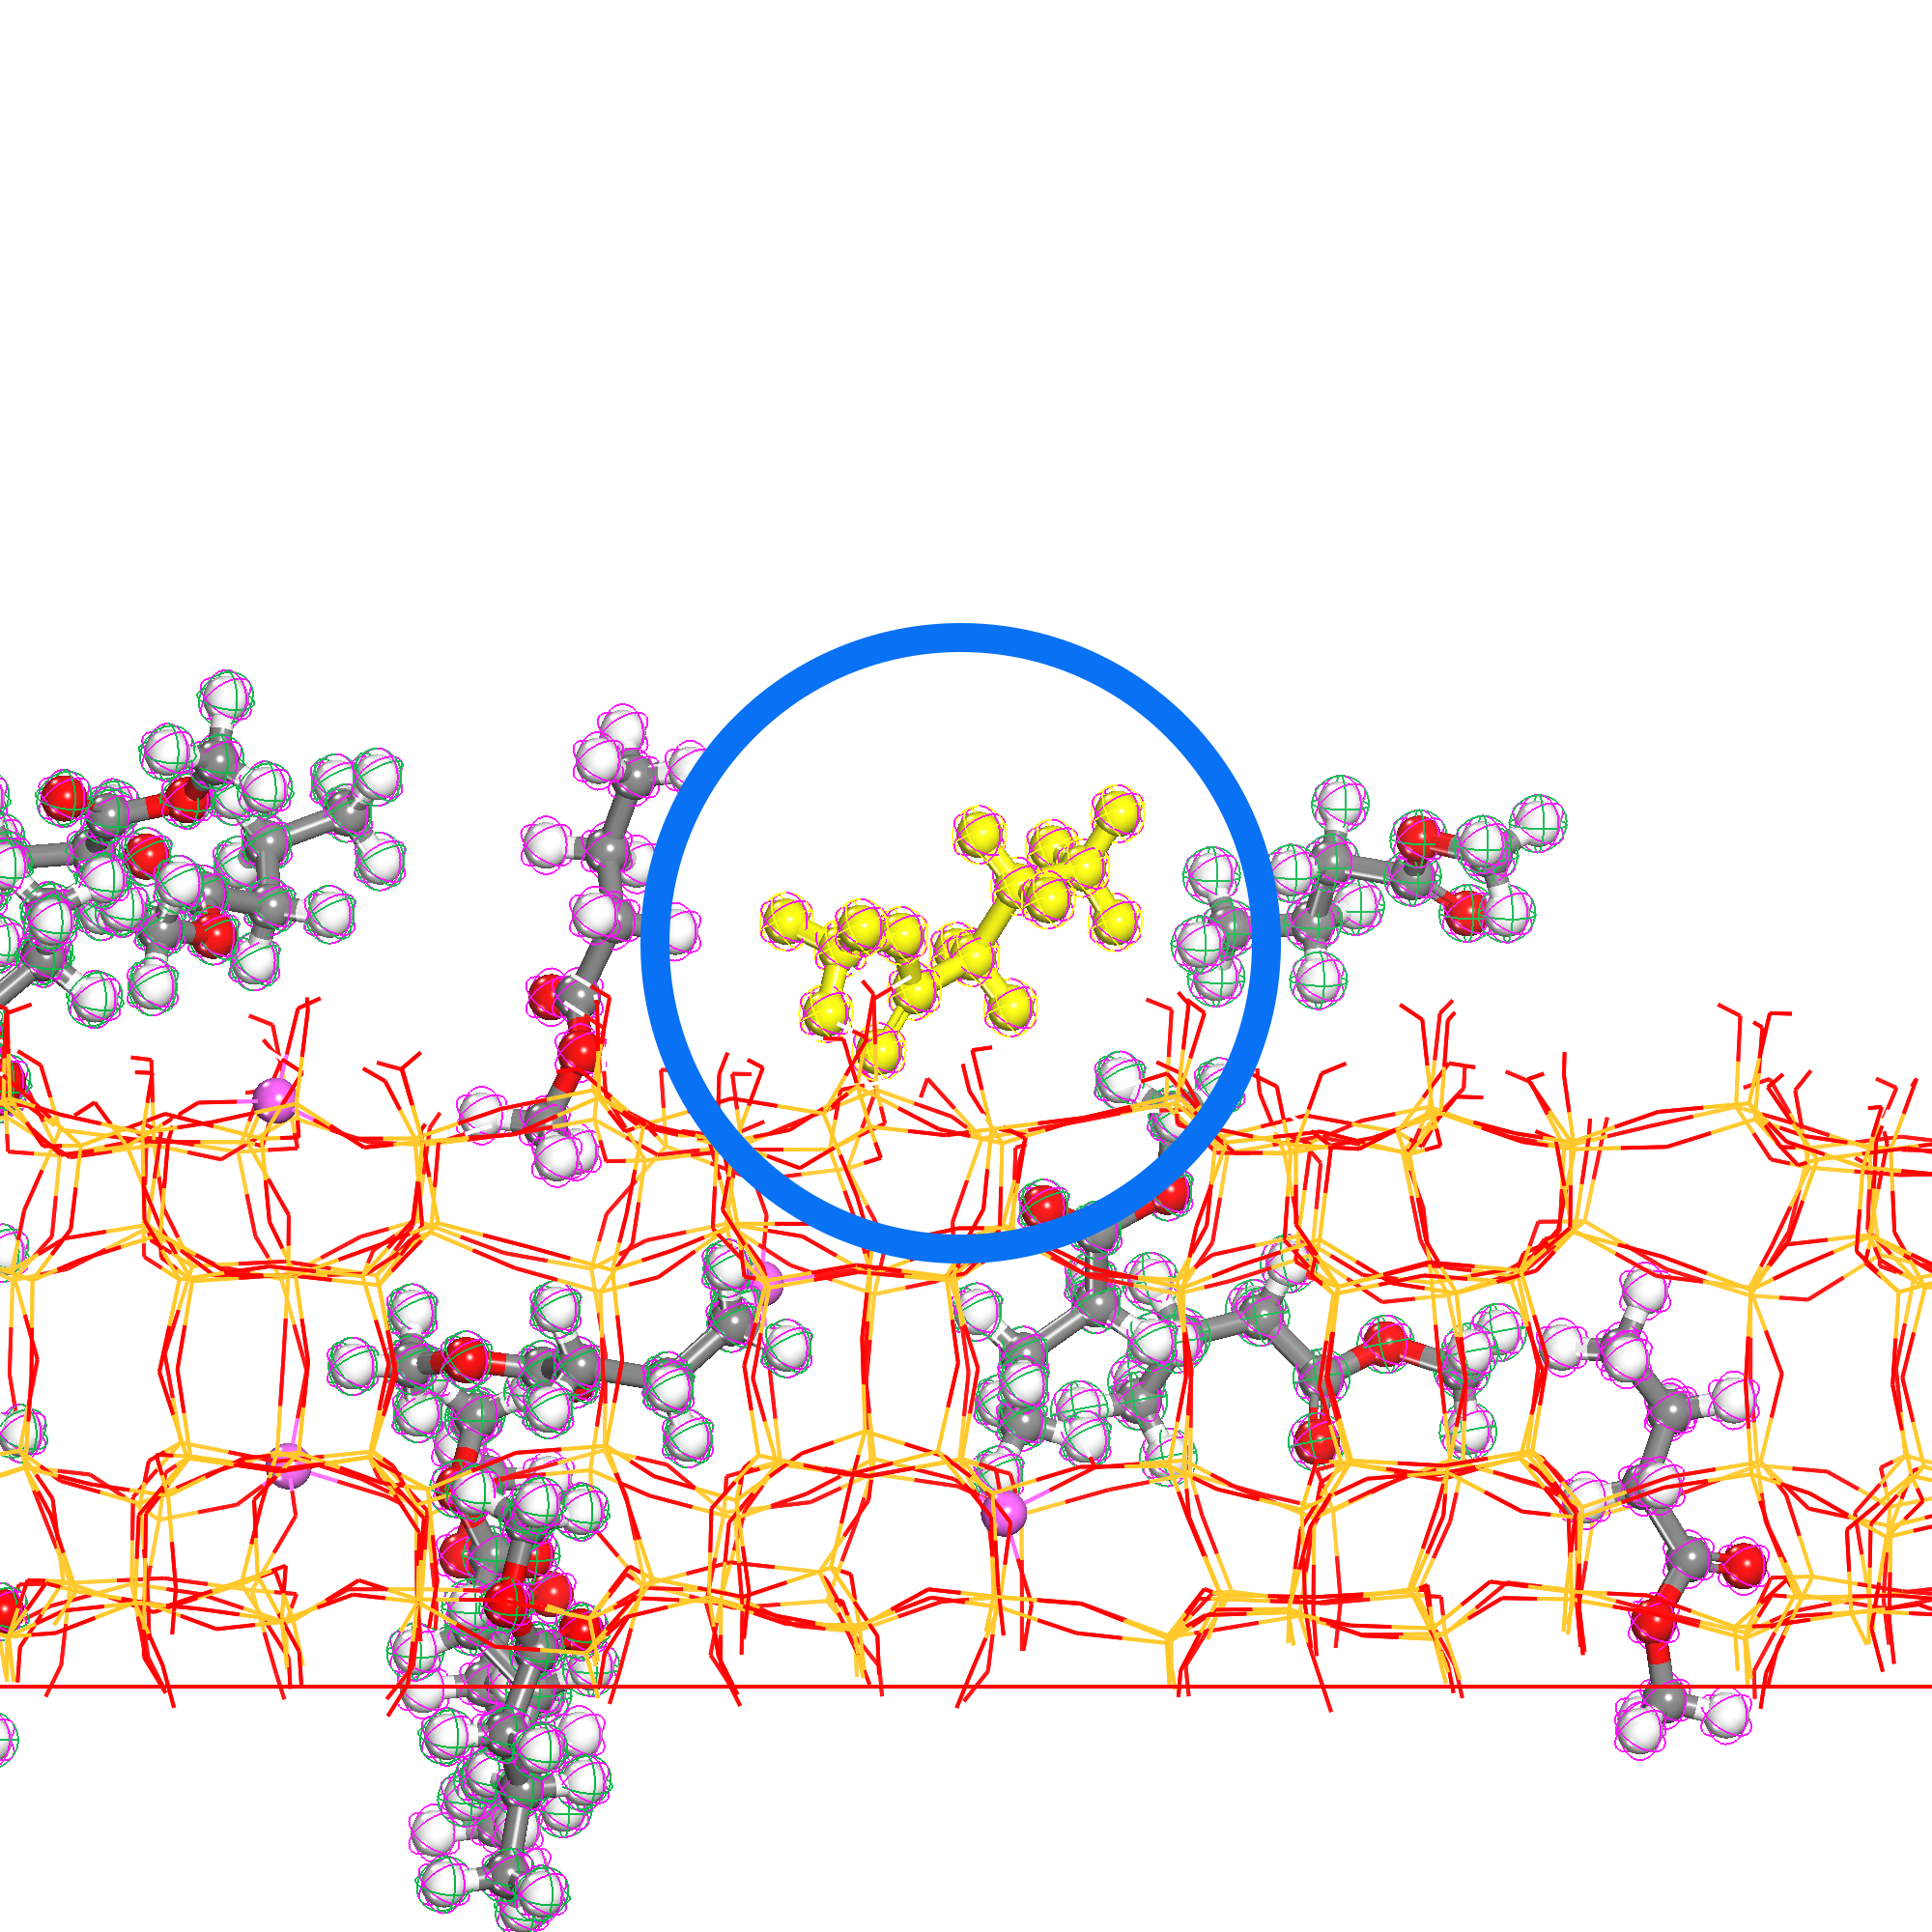
\includegraphics[width=1.35in]{figure/Diffusion/7.png}
    \end{minipage}%
    }%
    \subfigure[35ps]{
    \begin{minipage}[t]{0.25\linewidth}
    \centering
    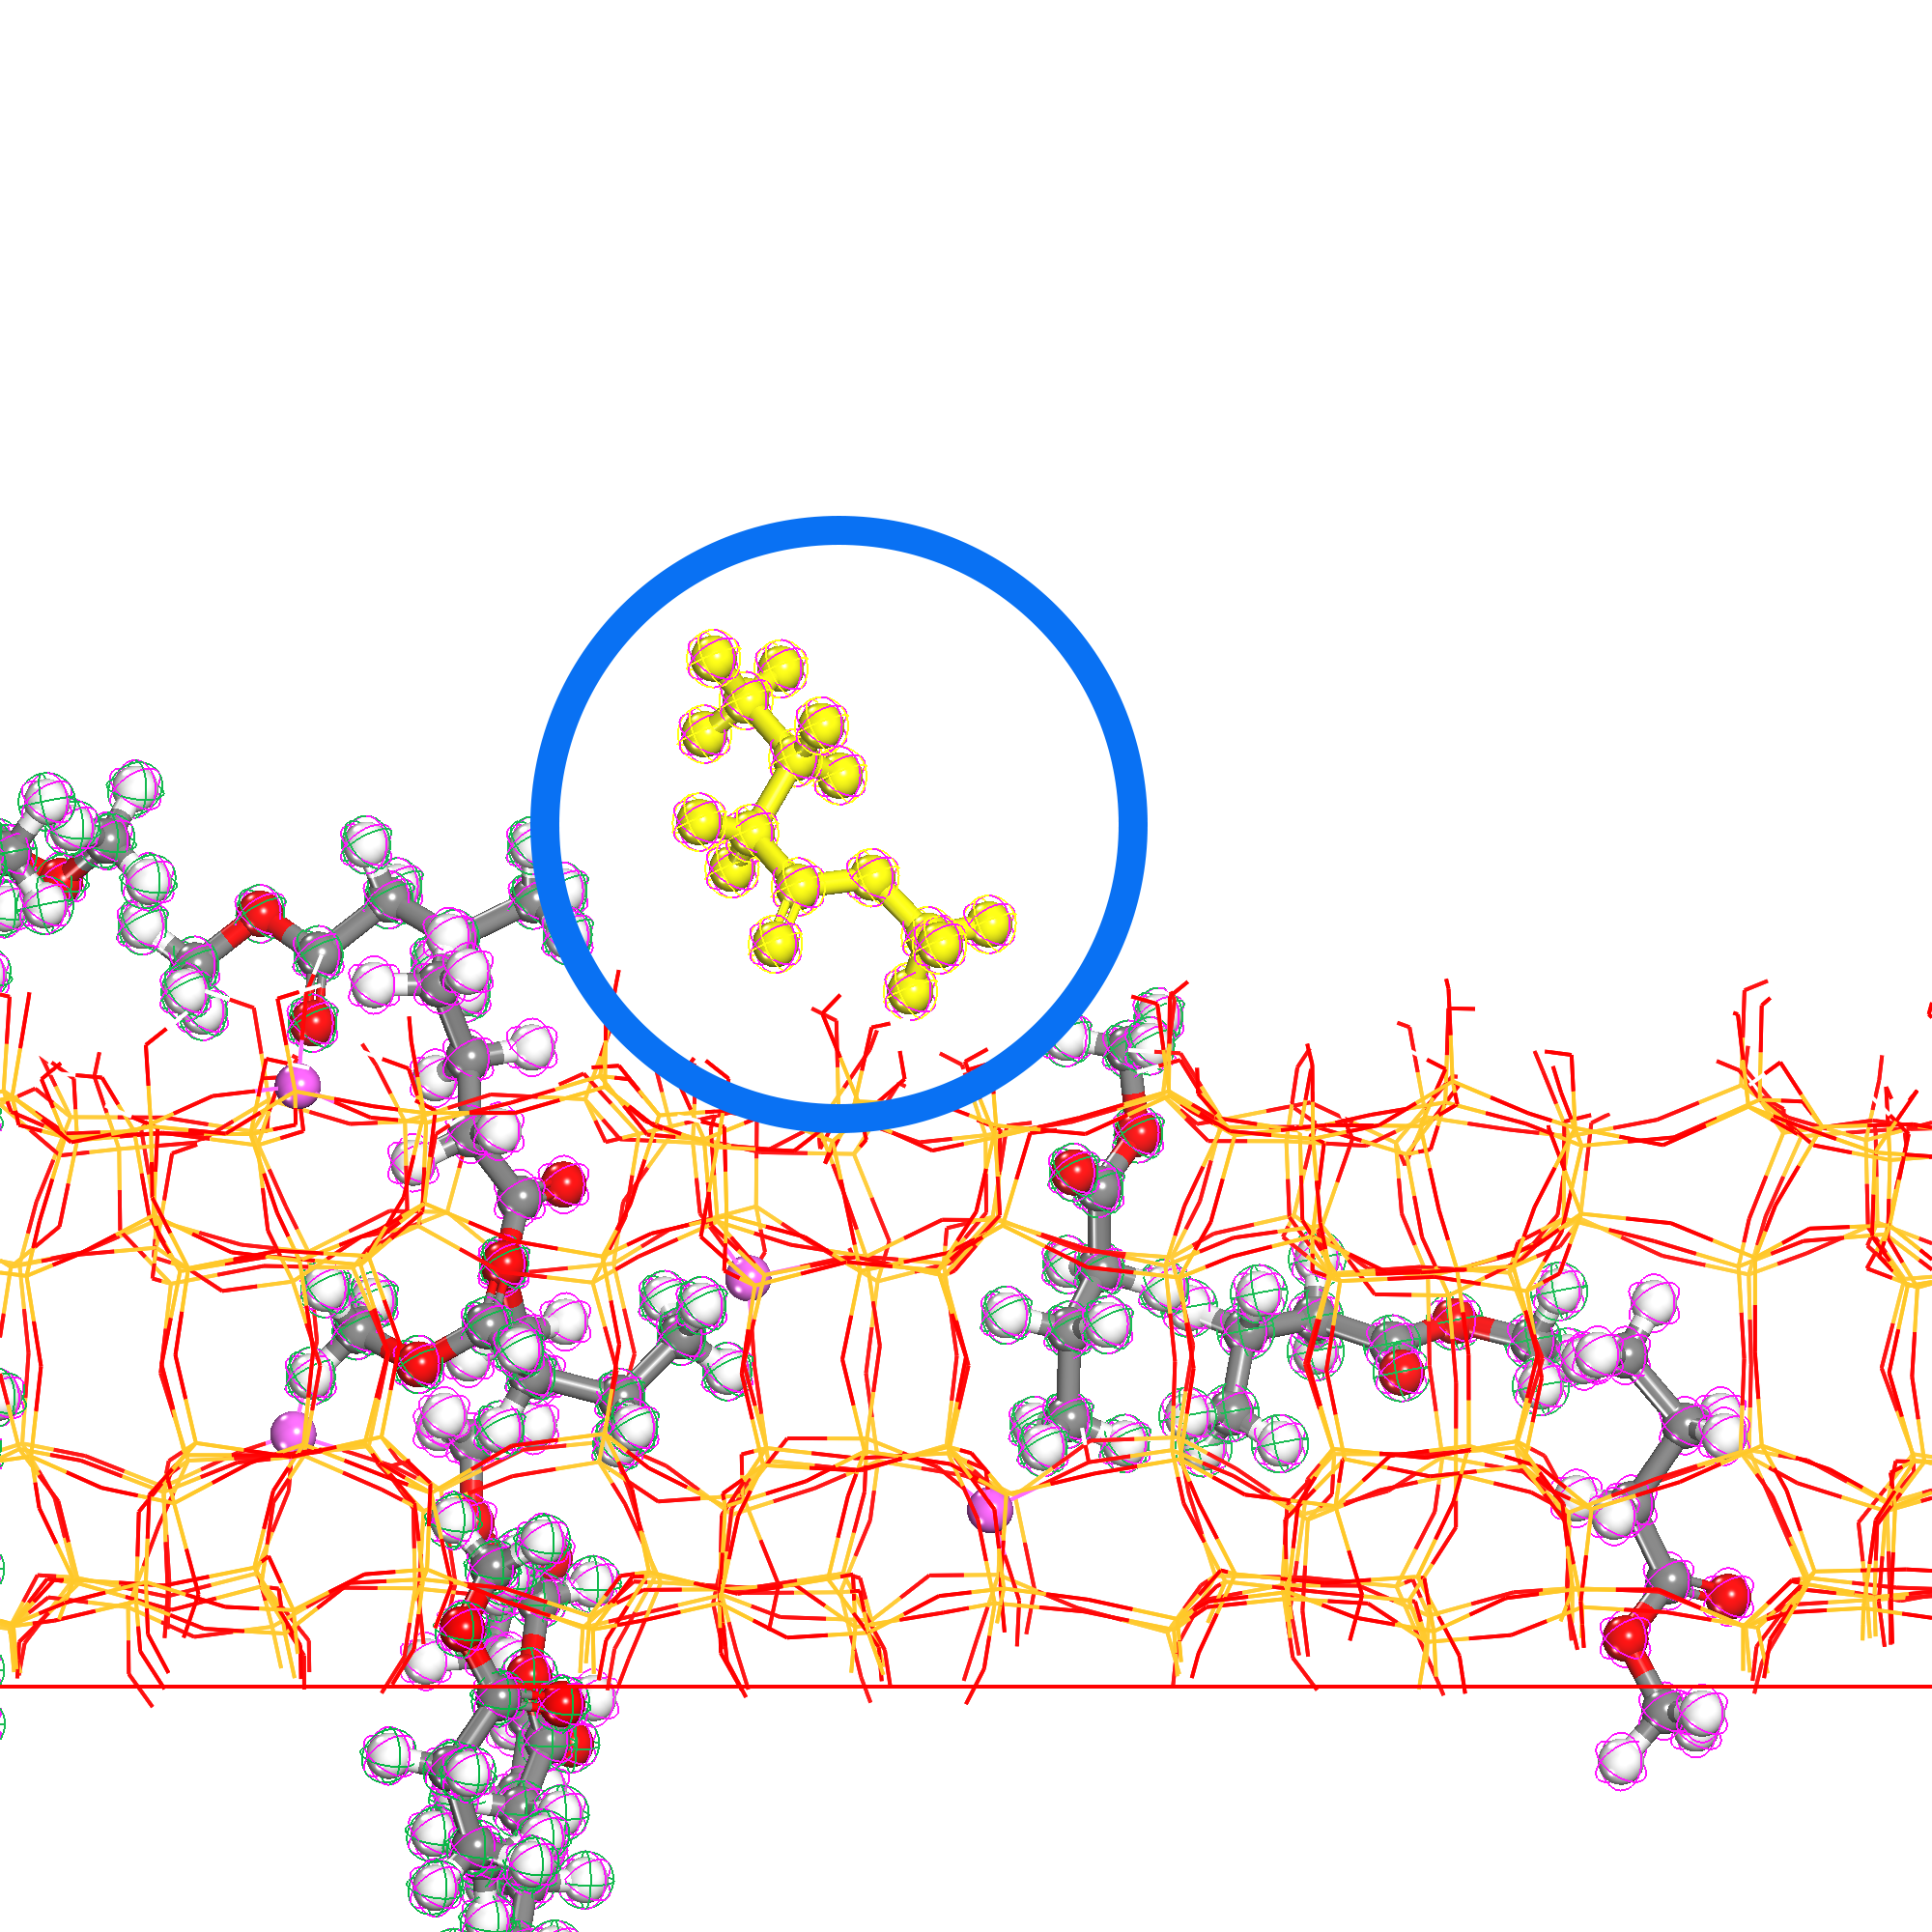
\includegraphics[width=1.35in]{figure/Diffusion/8.png}
    %\caption{fig2}
    \end{minipage}%
    }%

    \caption{丁酸甲酯在60Å介孔的H-ZSM-5分子筛的扩散轨迹随时间变化图}
    \label{fig:MSDa}
\end{figure}
\par{\reffig{fig:MSDa}清楚地展示了丁酸甲酯分子因为取向与微孔孔道方向不一样而被弹开的过程。而\reffig{fig:MSDf}展示了当丁酸甲酯的取向与微孔孔道一致时,丁酸甲酯顺利地进入A方向的之字形微孔内的过程。这进一步说明H-ZSM-5分子筛具有很高的择形性。}
\begin{figure}[H]
    \centering

    \subfigure[80ps]{
    \begin{minipage}[t]{0.25\linewidth}
    \centering
    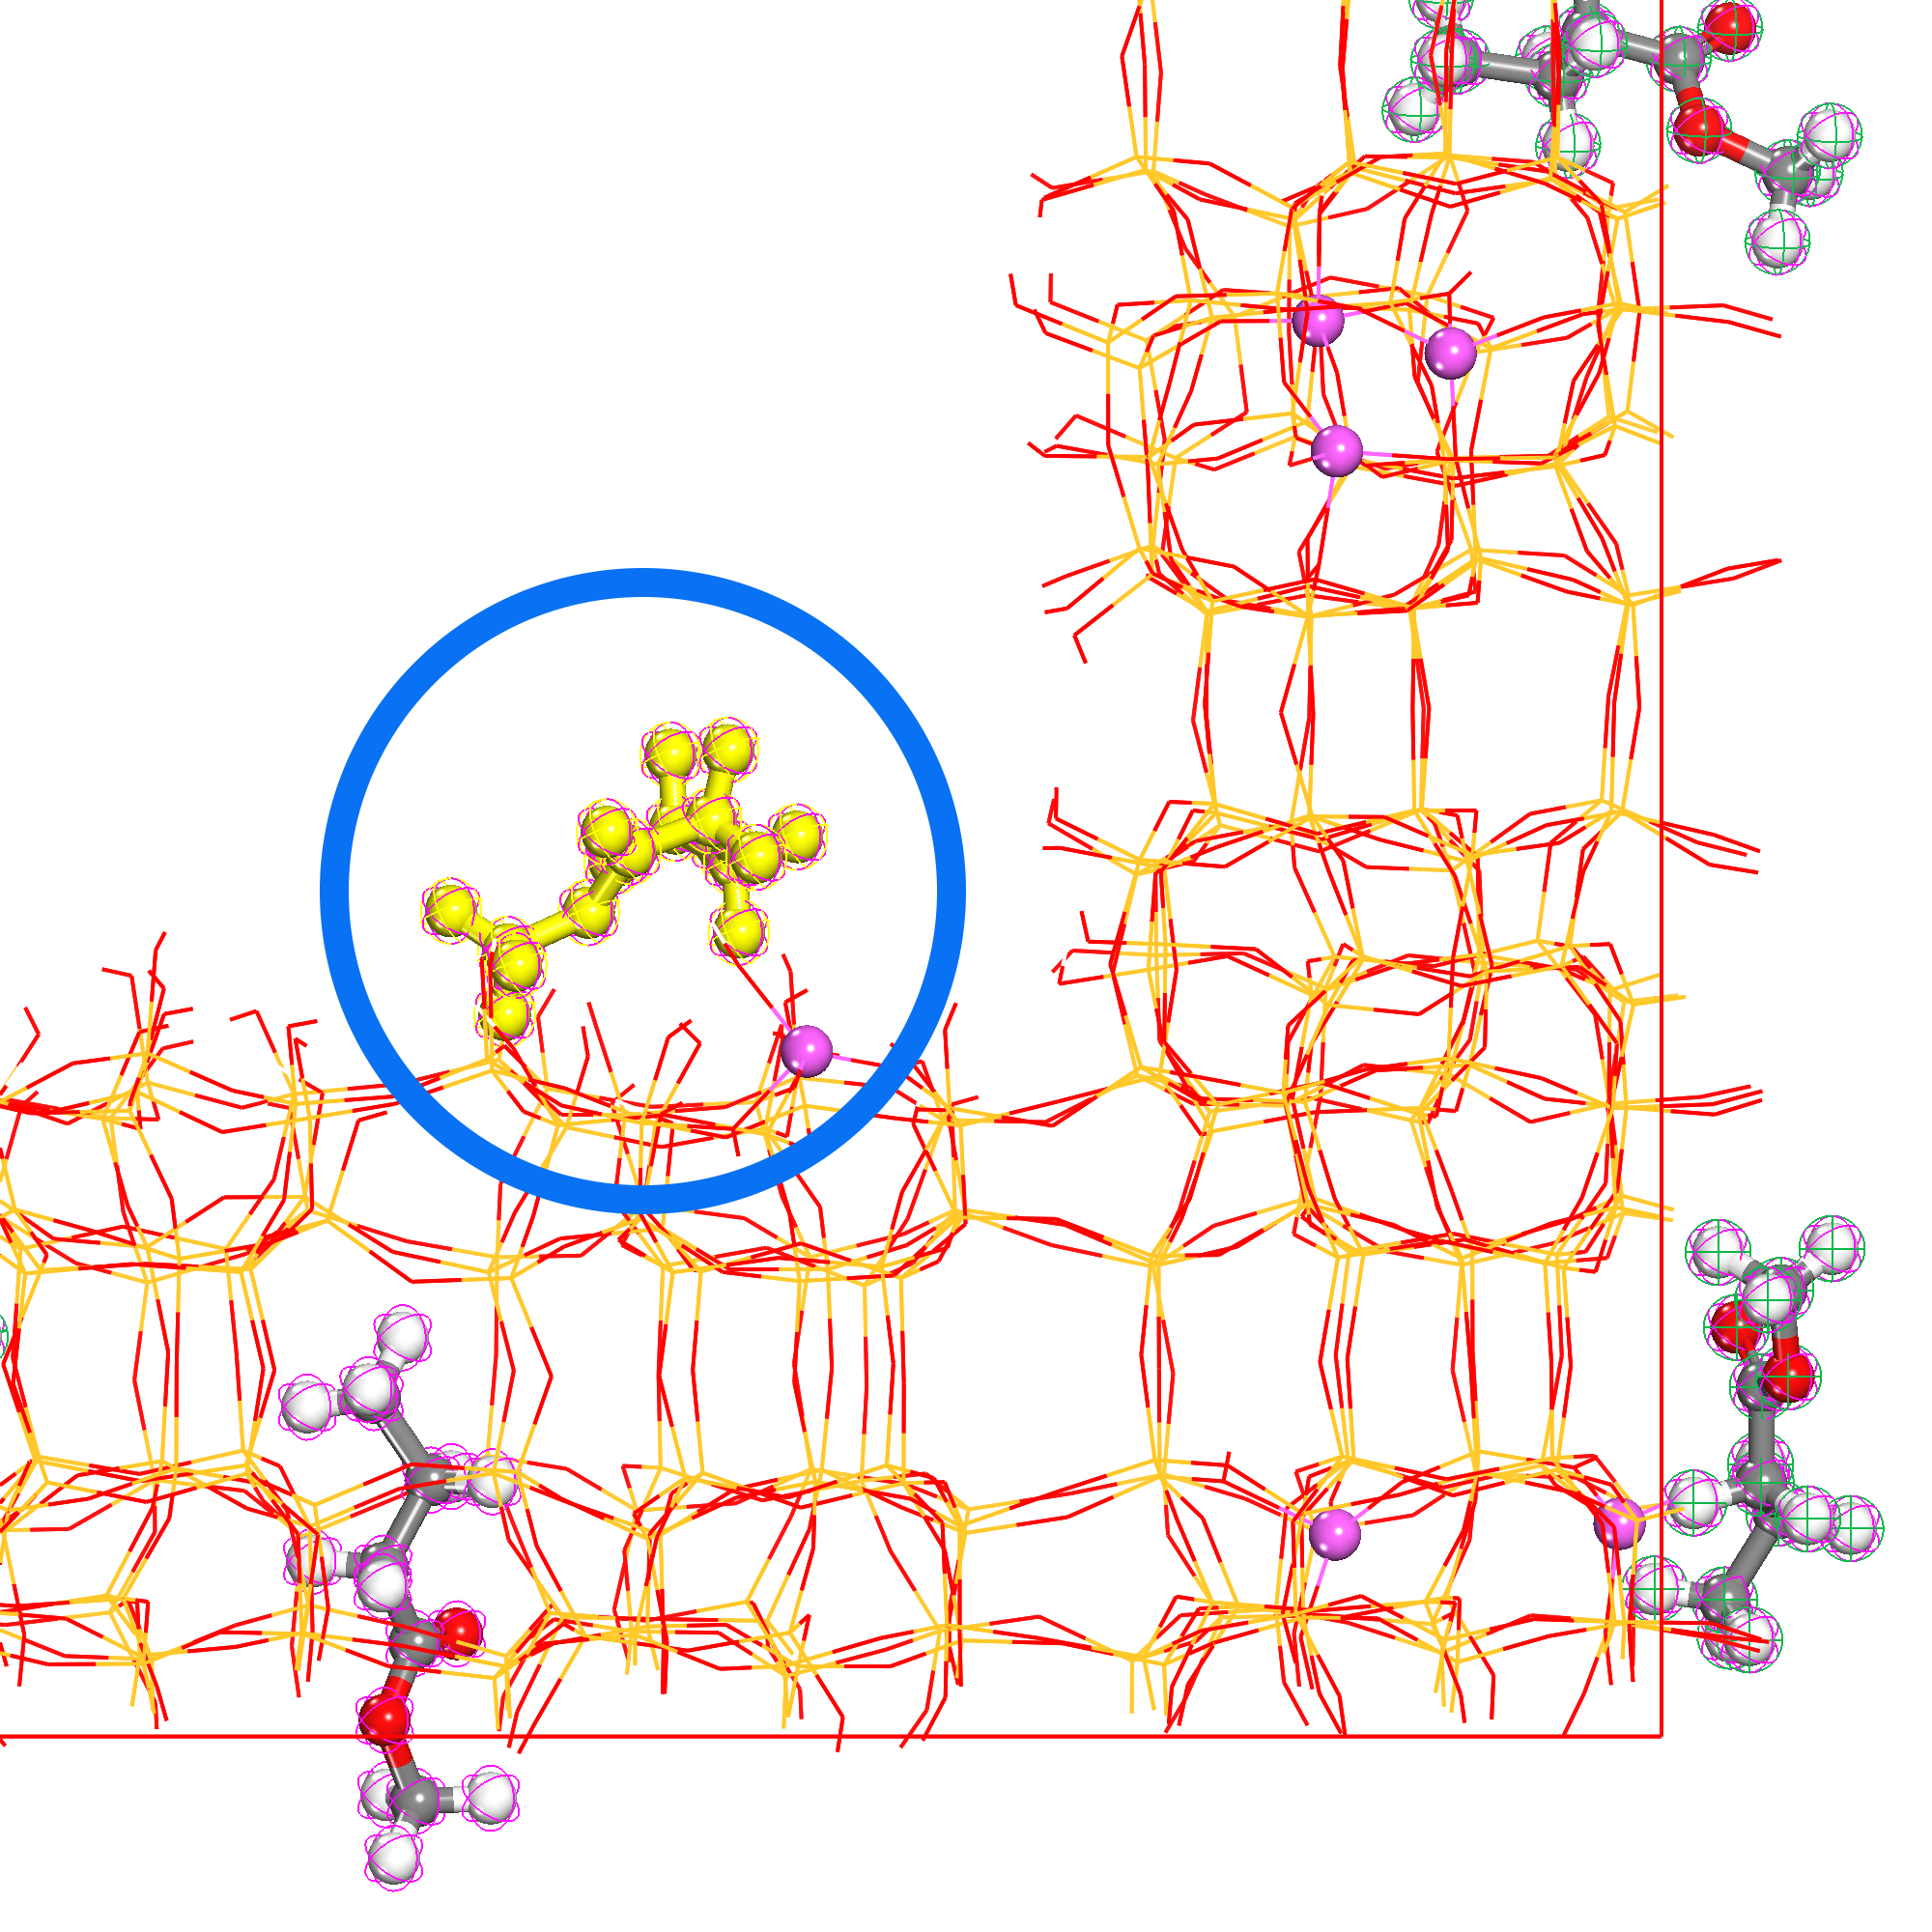
\includegraphics[width=1.35in]{figure/Diffusion/1new.png}
    \end{minipage}%
    }%
    \subfigure[85ps]{
    \begin{minipage}[t]{0.25\linewidth}
    \centering
    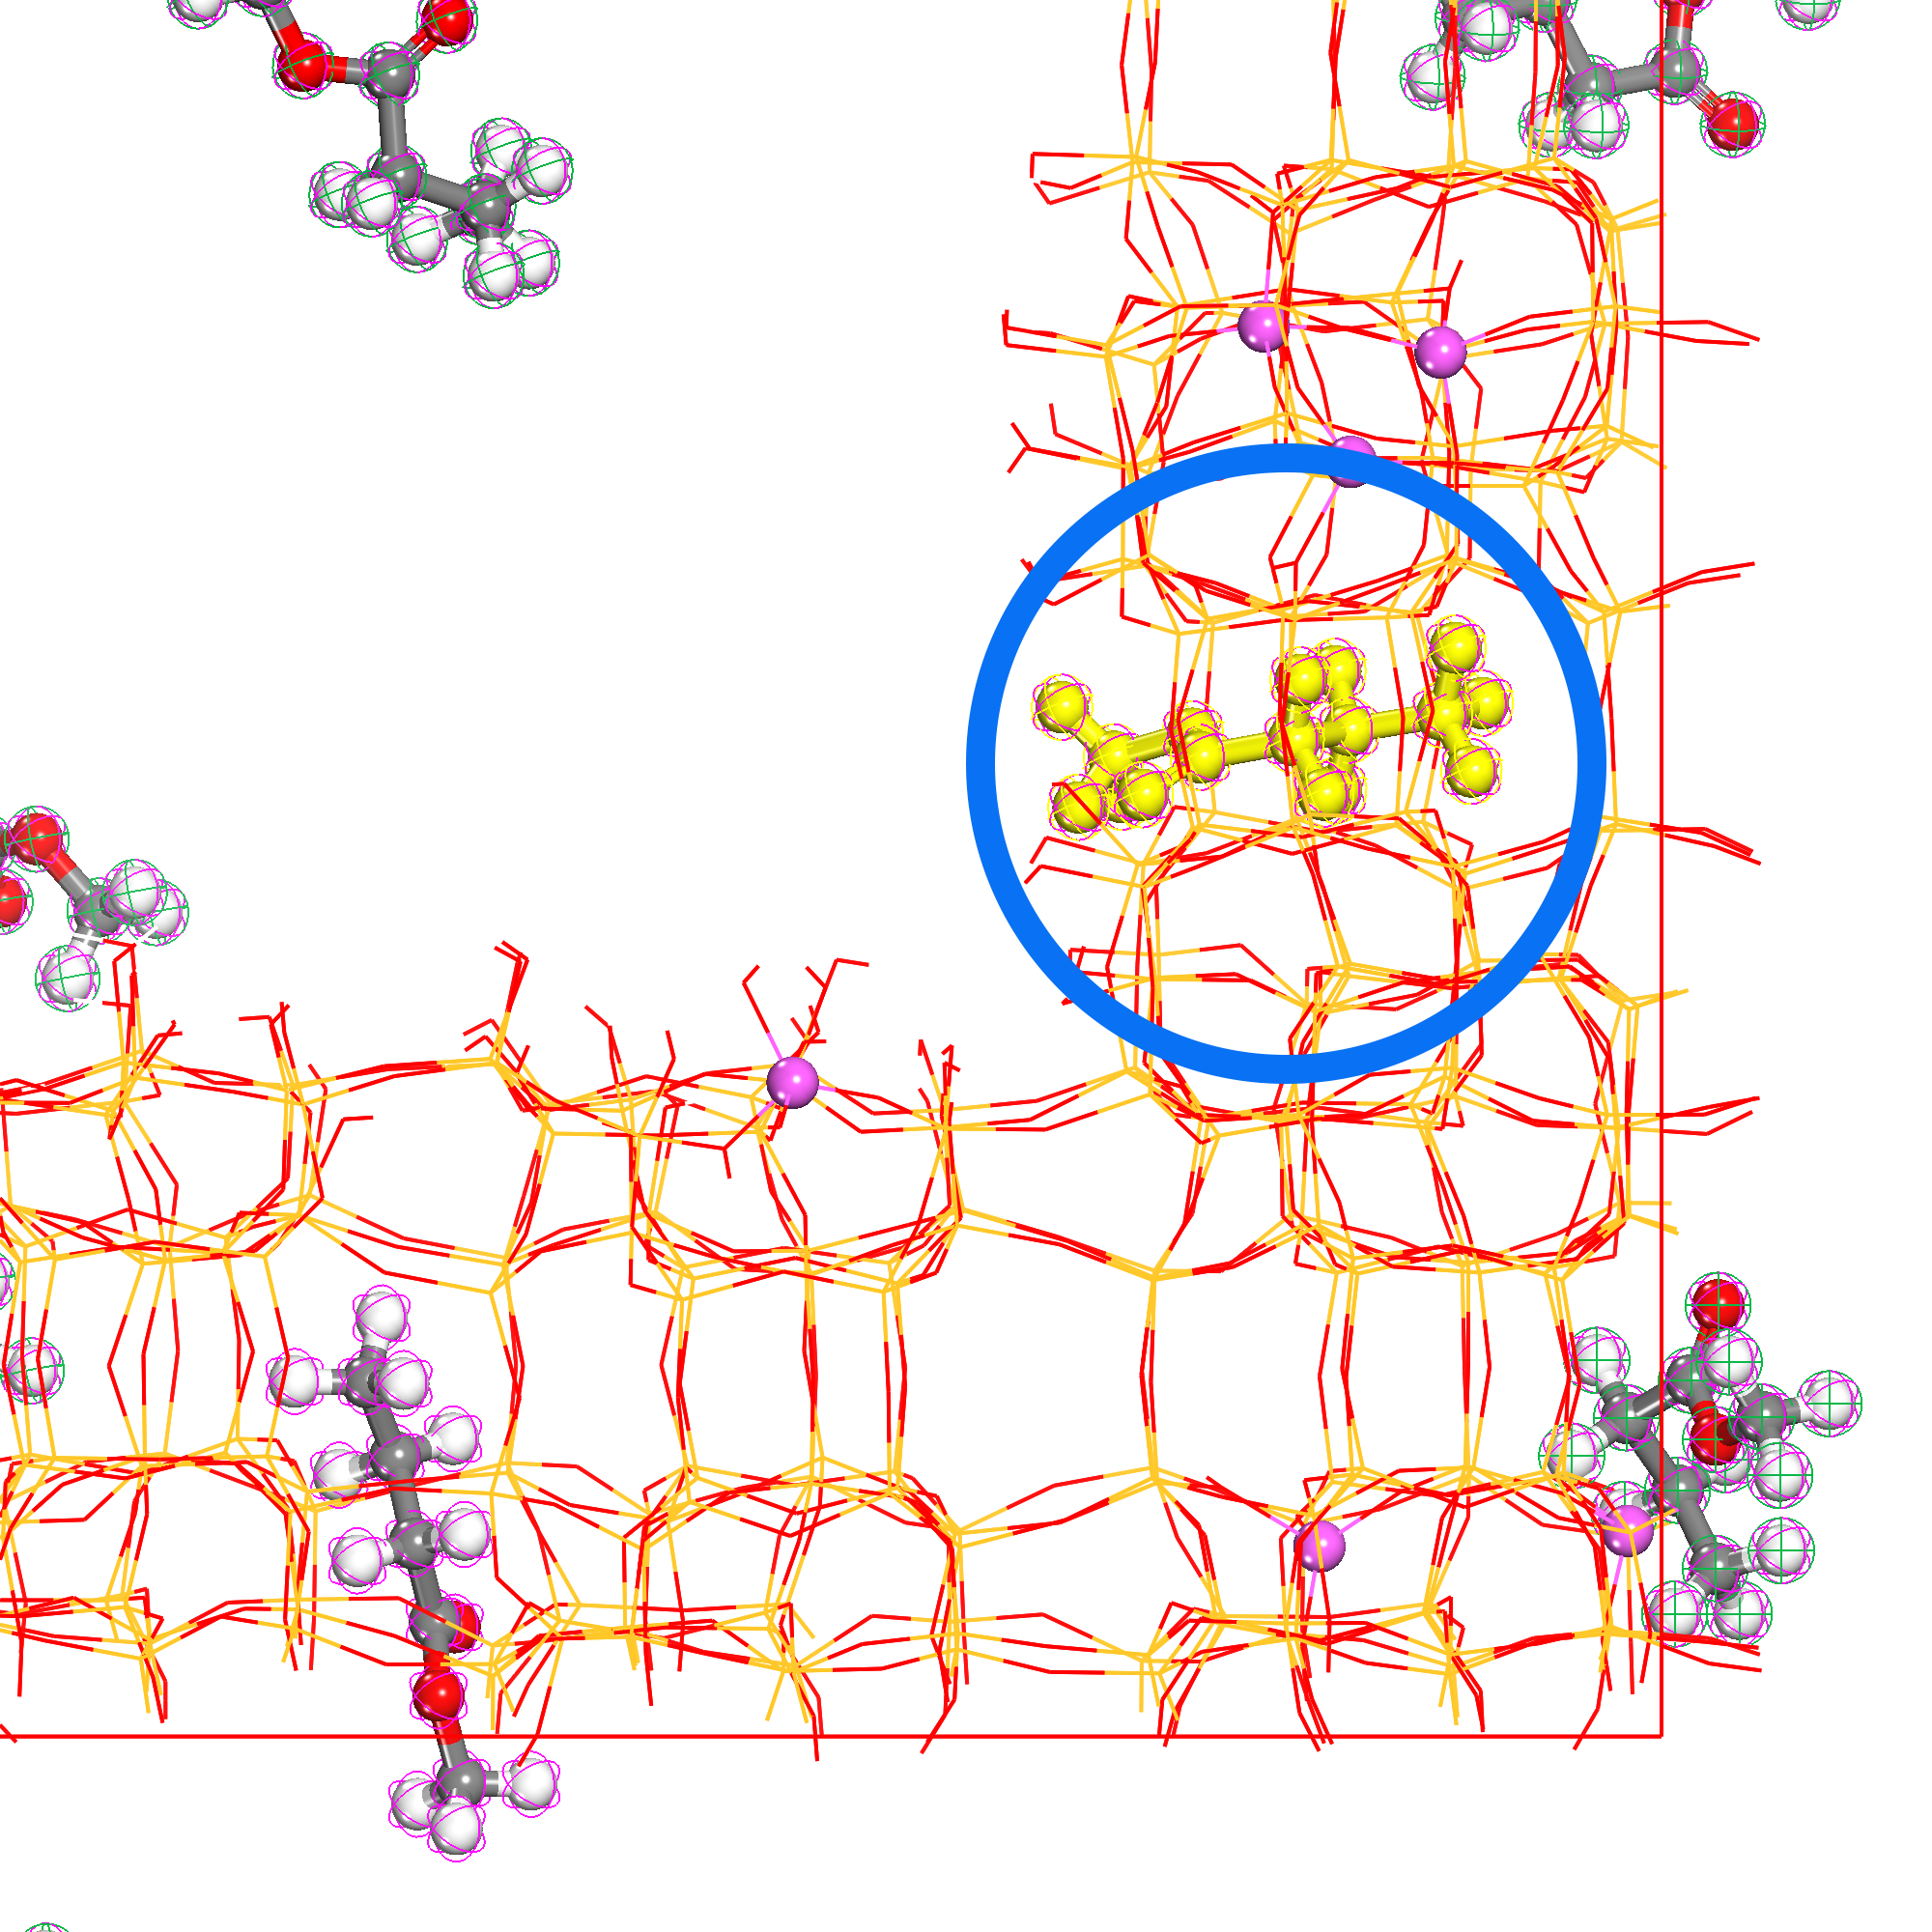
\includegraphics[width=1.35in]{figure/Diffusion/2new.png}
    %\caption{fig2}
    \end{minipage}%
    }%
    \subfigure[90ps]{
    \begin{minipage}[t]{0.25\linewidth}
    \centering
    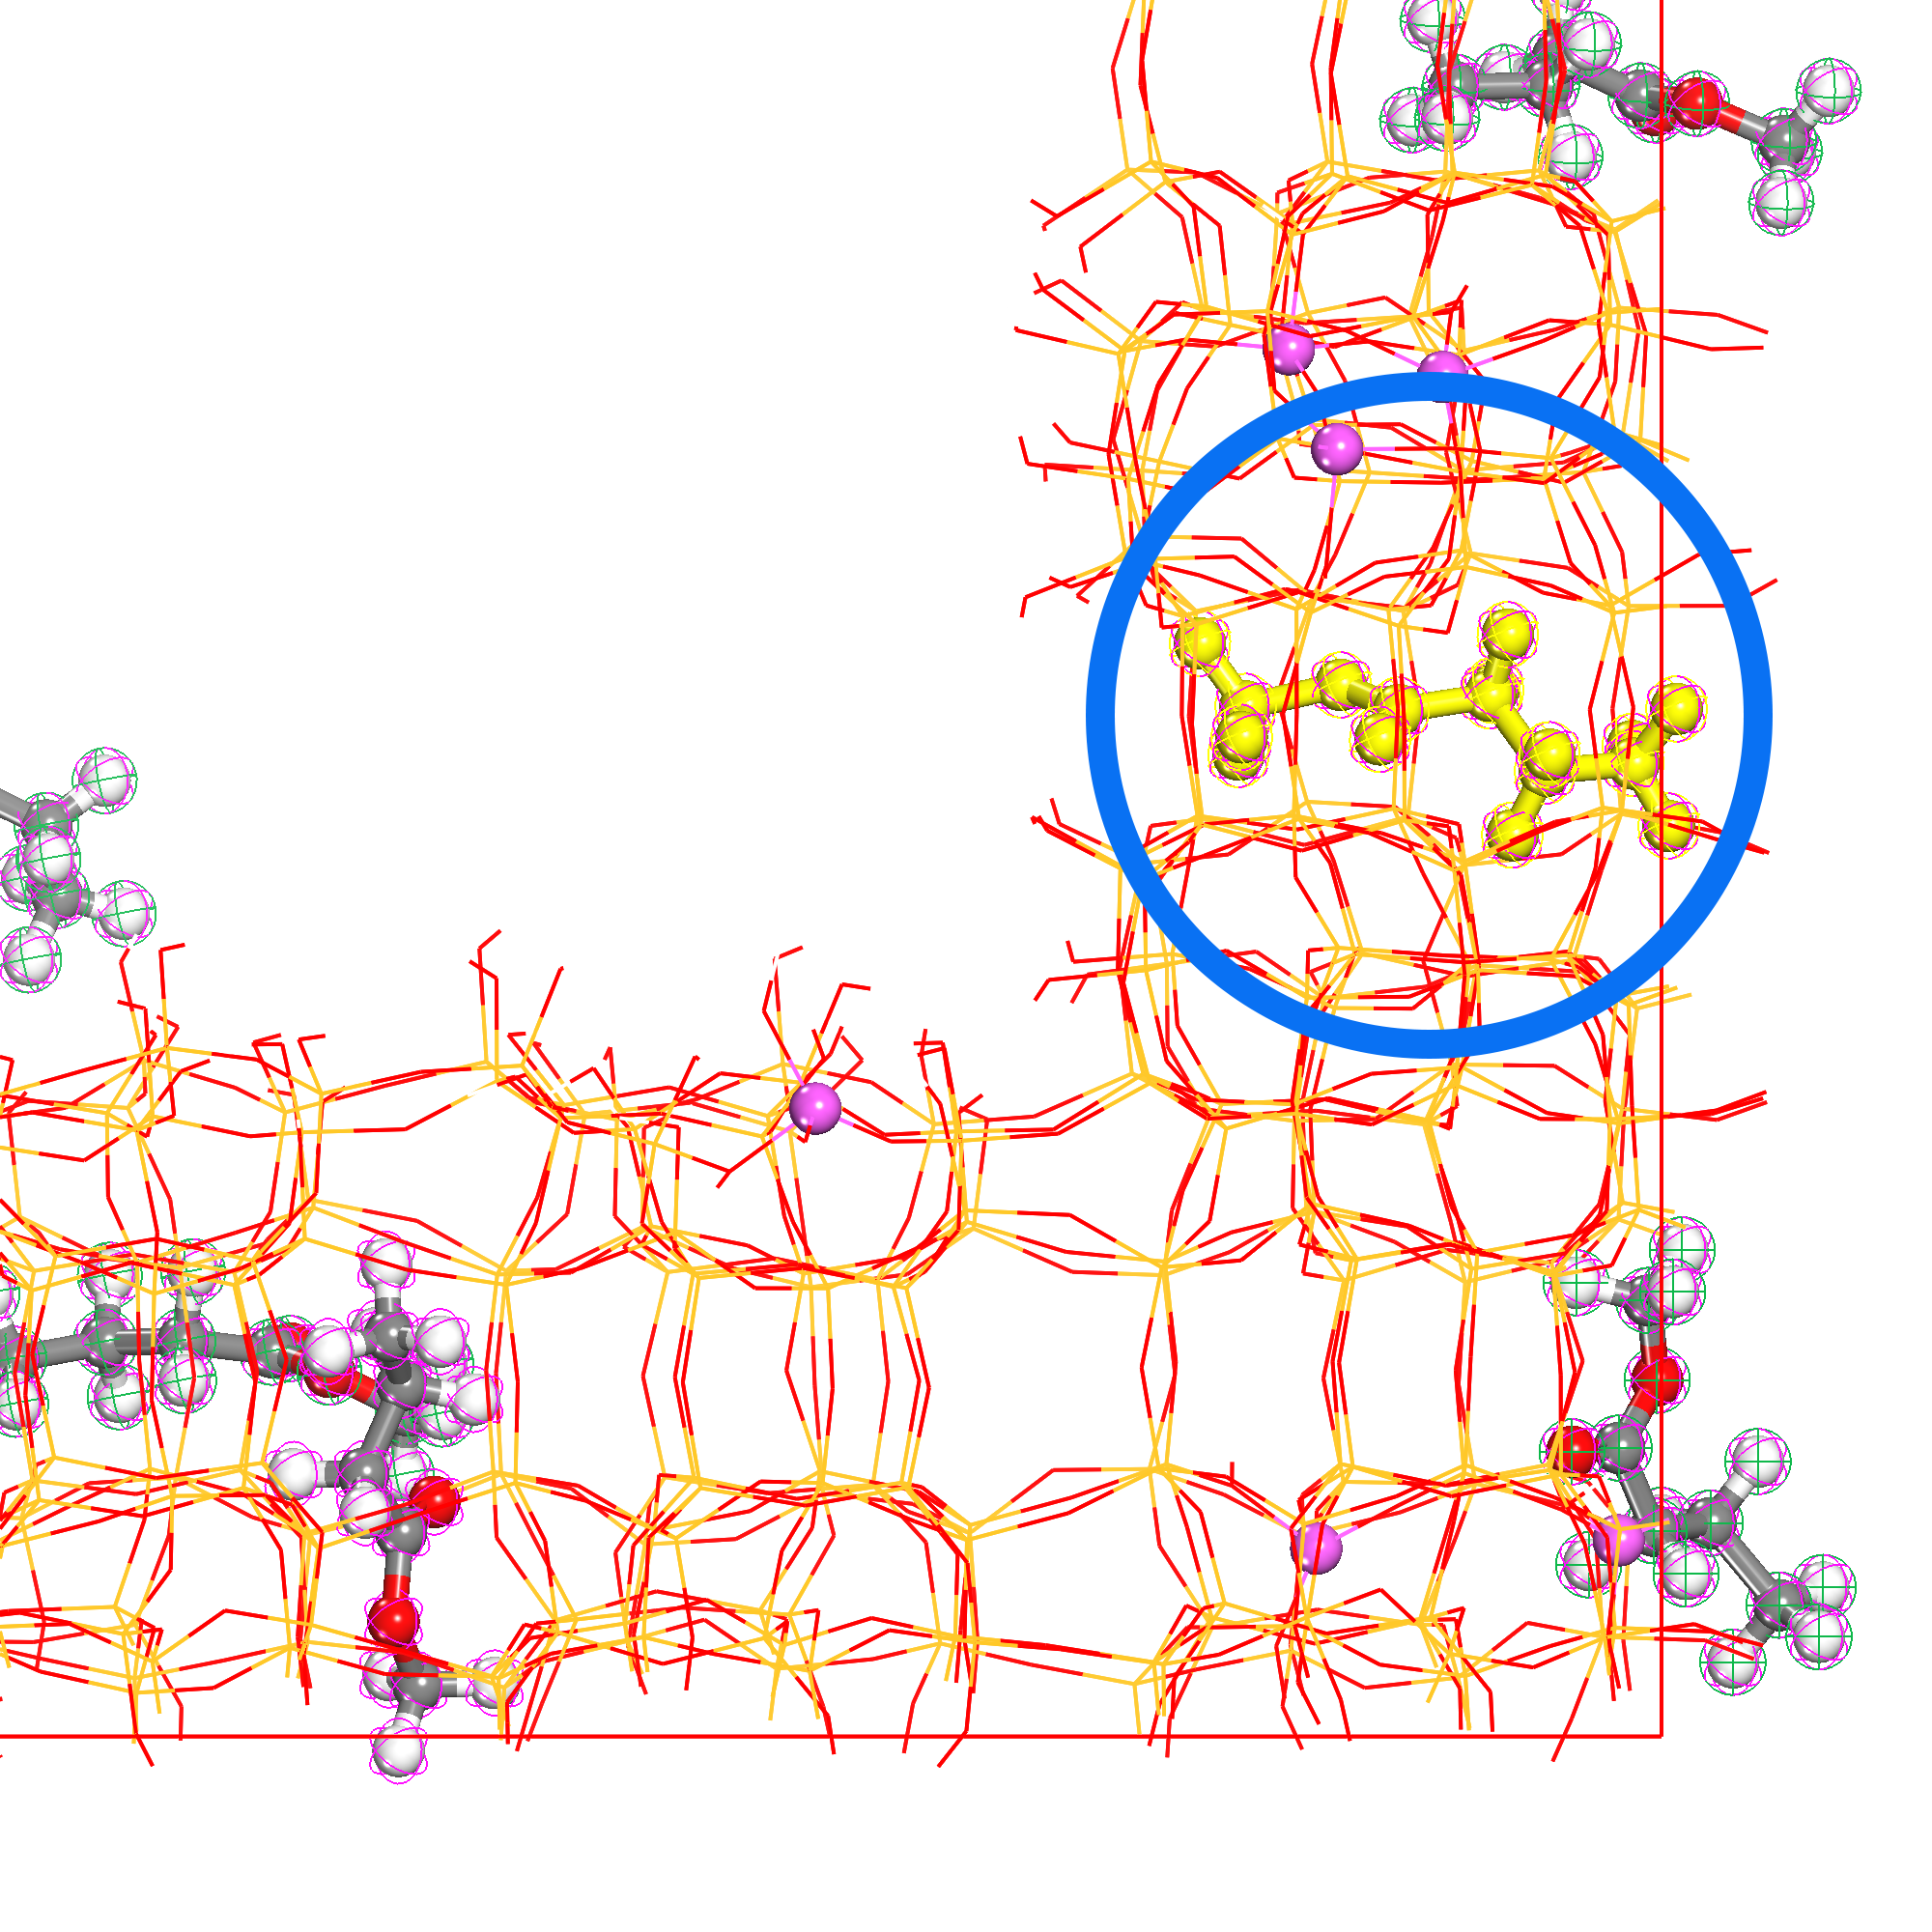
\includegraphics[width=1.35in]{figure/Diffusion/3new.png}
    %\caption{fig2}
    \end{minipage}%
    }%
    \subfigure[95ps]{
    \begin{minipage}[t]{0.25\linewidth}
    \centering
    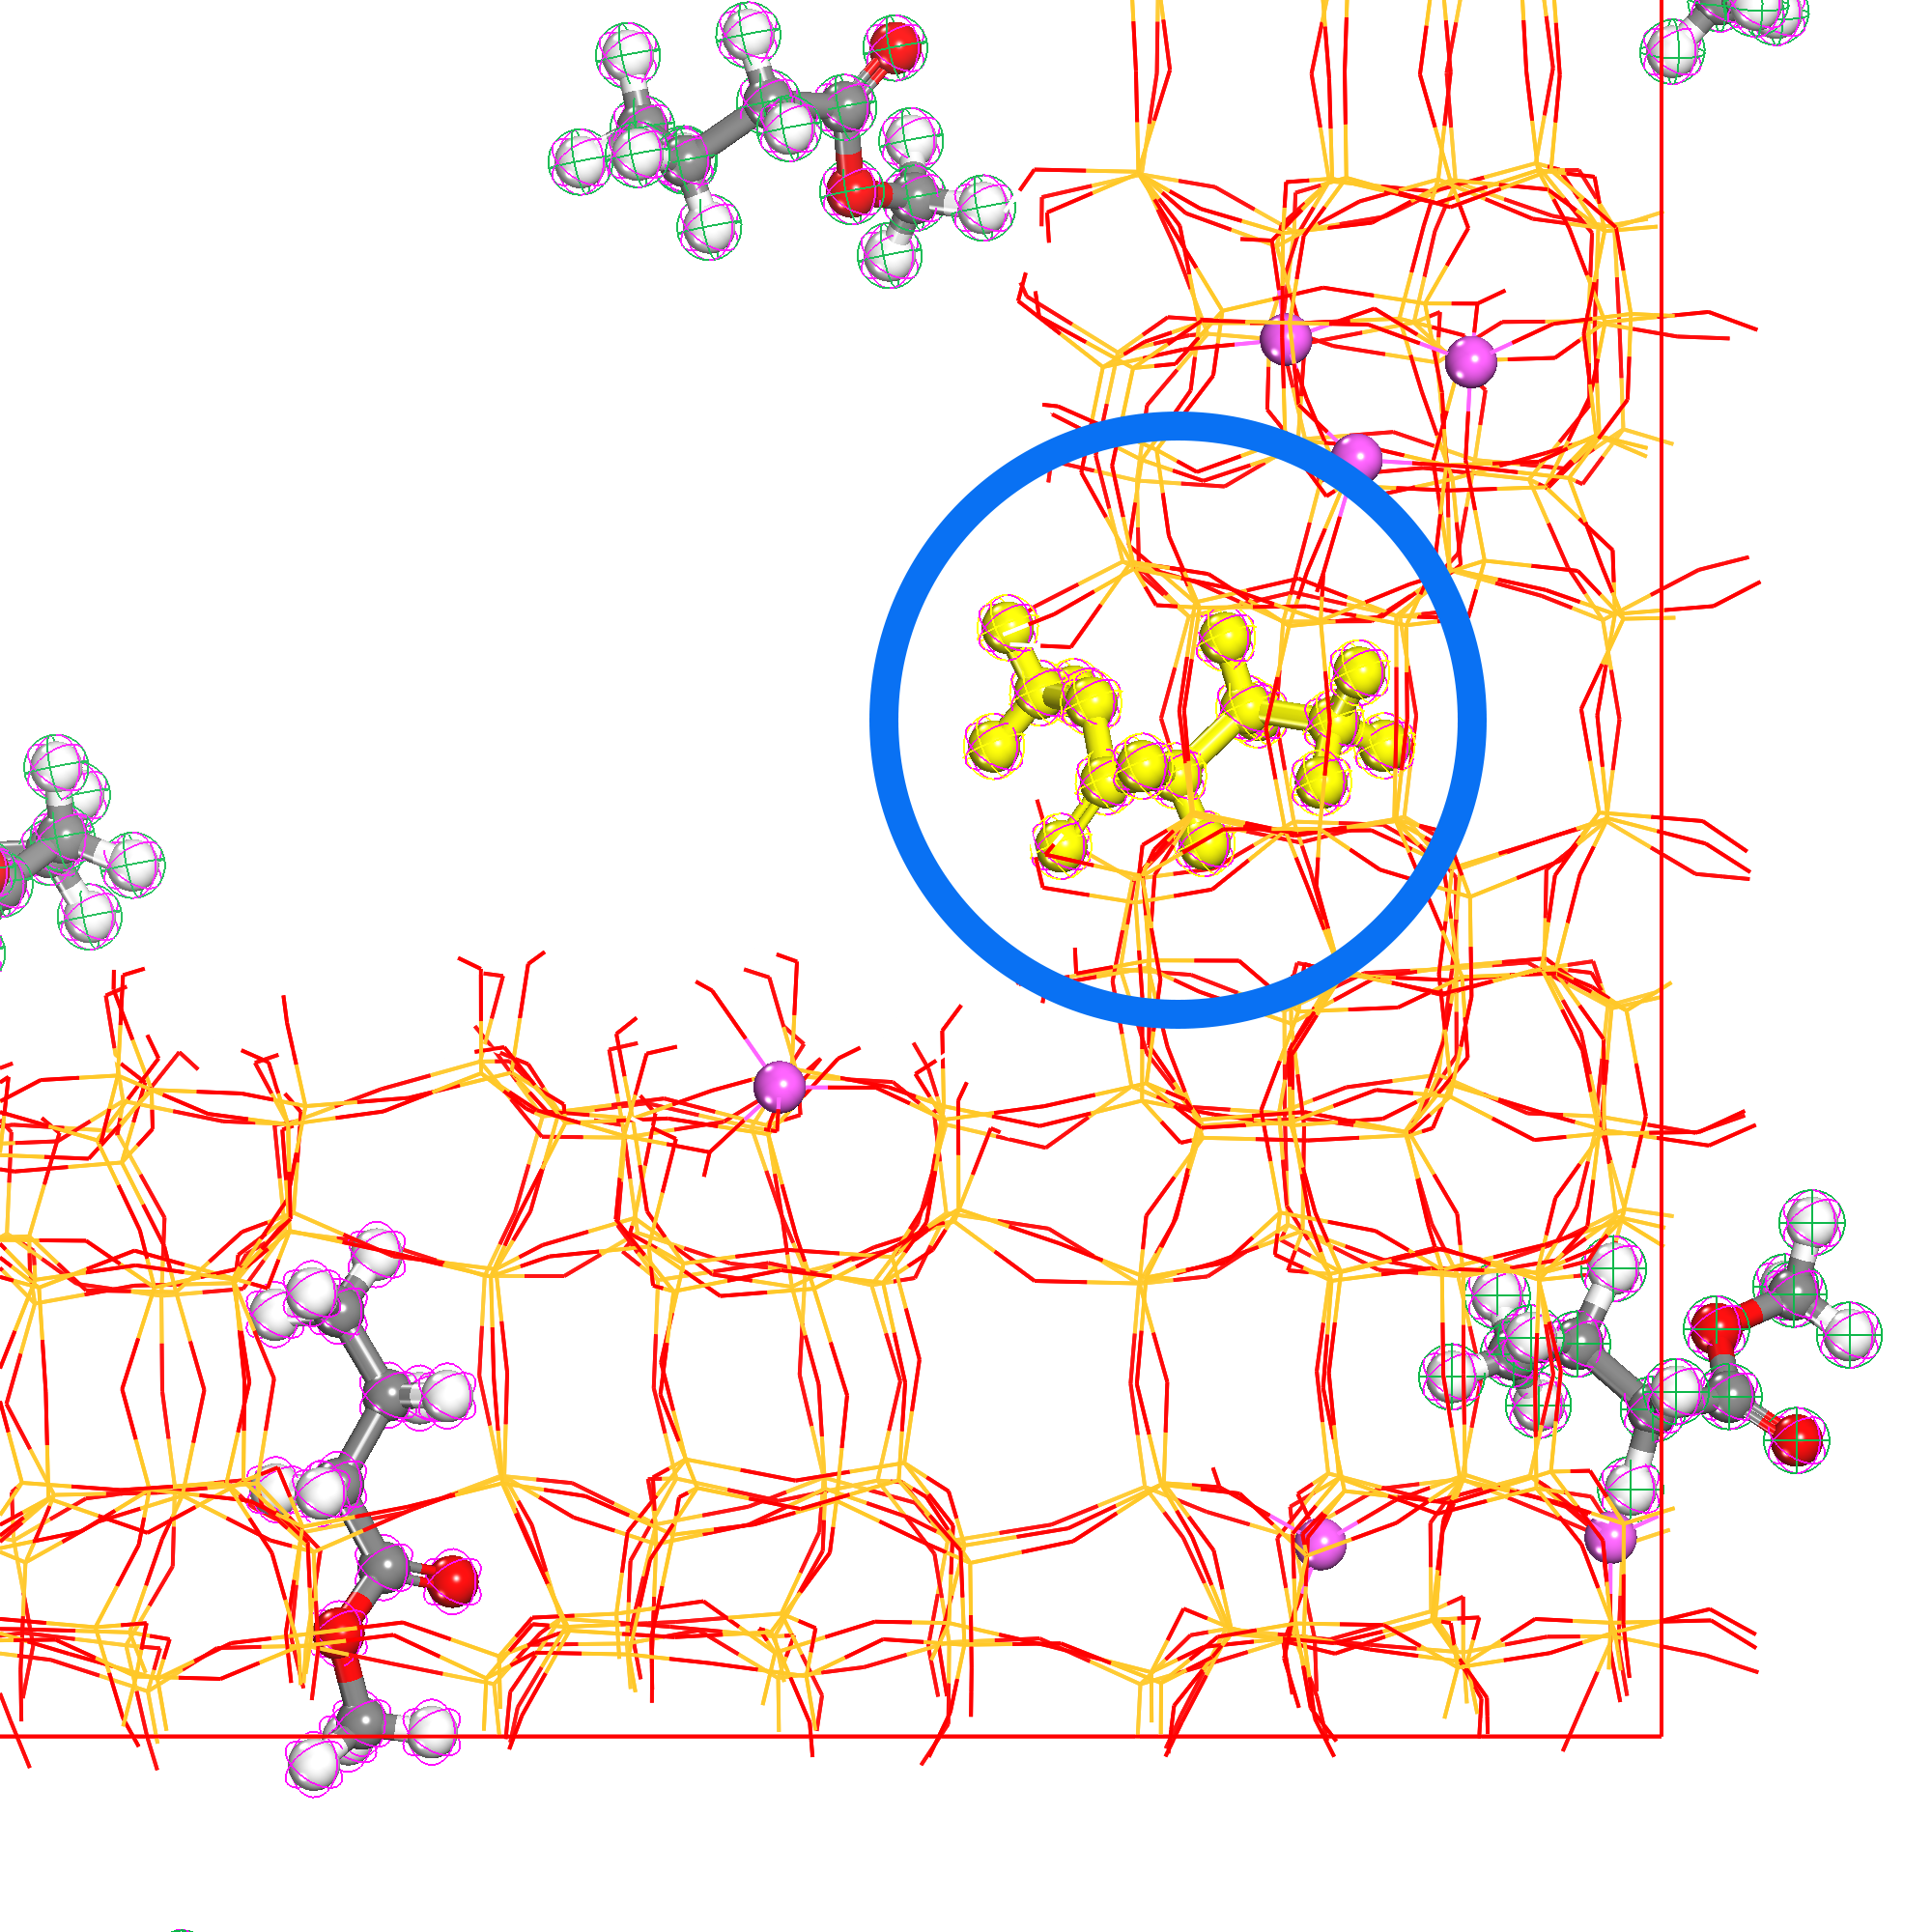
\includegraphics[width=1.35in]{figure/Diffusion/4new.png}
    \end{minipage}%
    }%
    \caption{丁酸甲酯从介孔到微孔的扩散轨迹随时间变化图}
    \label{fig:MSDf}
\end{figure}

\subsubsection{丁酸甲酯在微孔内的扩散}
\par{本小节主要讨论了丁酸甲酯进入微孔内的情况。}
\par{为了更好地说明吸附分子从介孔进入微孔后,吸附分子在微孔内的扩散情况,本文将丁酸甲酯用Sorption模块的固定吸附的方式将丁酸甲酯固定在微孔内,并与微孔分子筛的结果进行对比。以分子筛的C方向为例,如\reffig{fig:MMe}所示}

\begin{figure}[H]
    \centering

    \subfigure[微孔]{
    \begin{minipage}[t]{0.3333\linewidth}
    \centering
    \includegraphics[width=1.8in]{figure/Diffusion/2MM.png}
    %\caption{fig1}
    \end{minipage}%
    }%
    \subfigure[20Å介孔]{
    \begin{minipage}[t]{0.3333\linewidth}
    \centering
    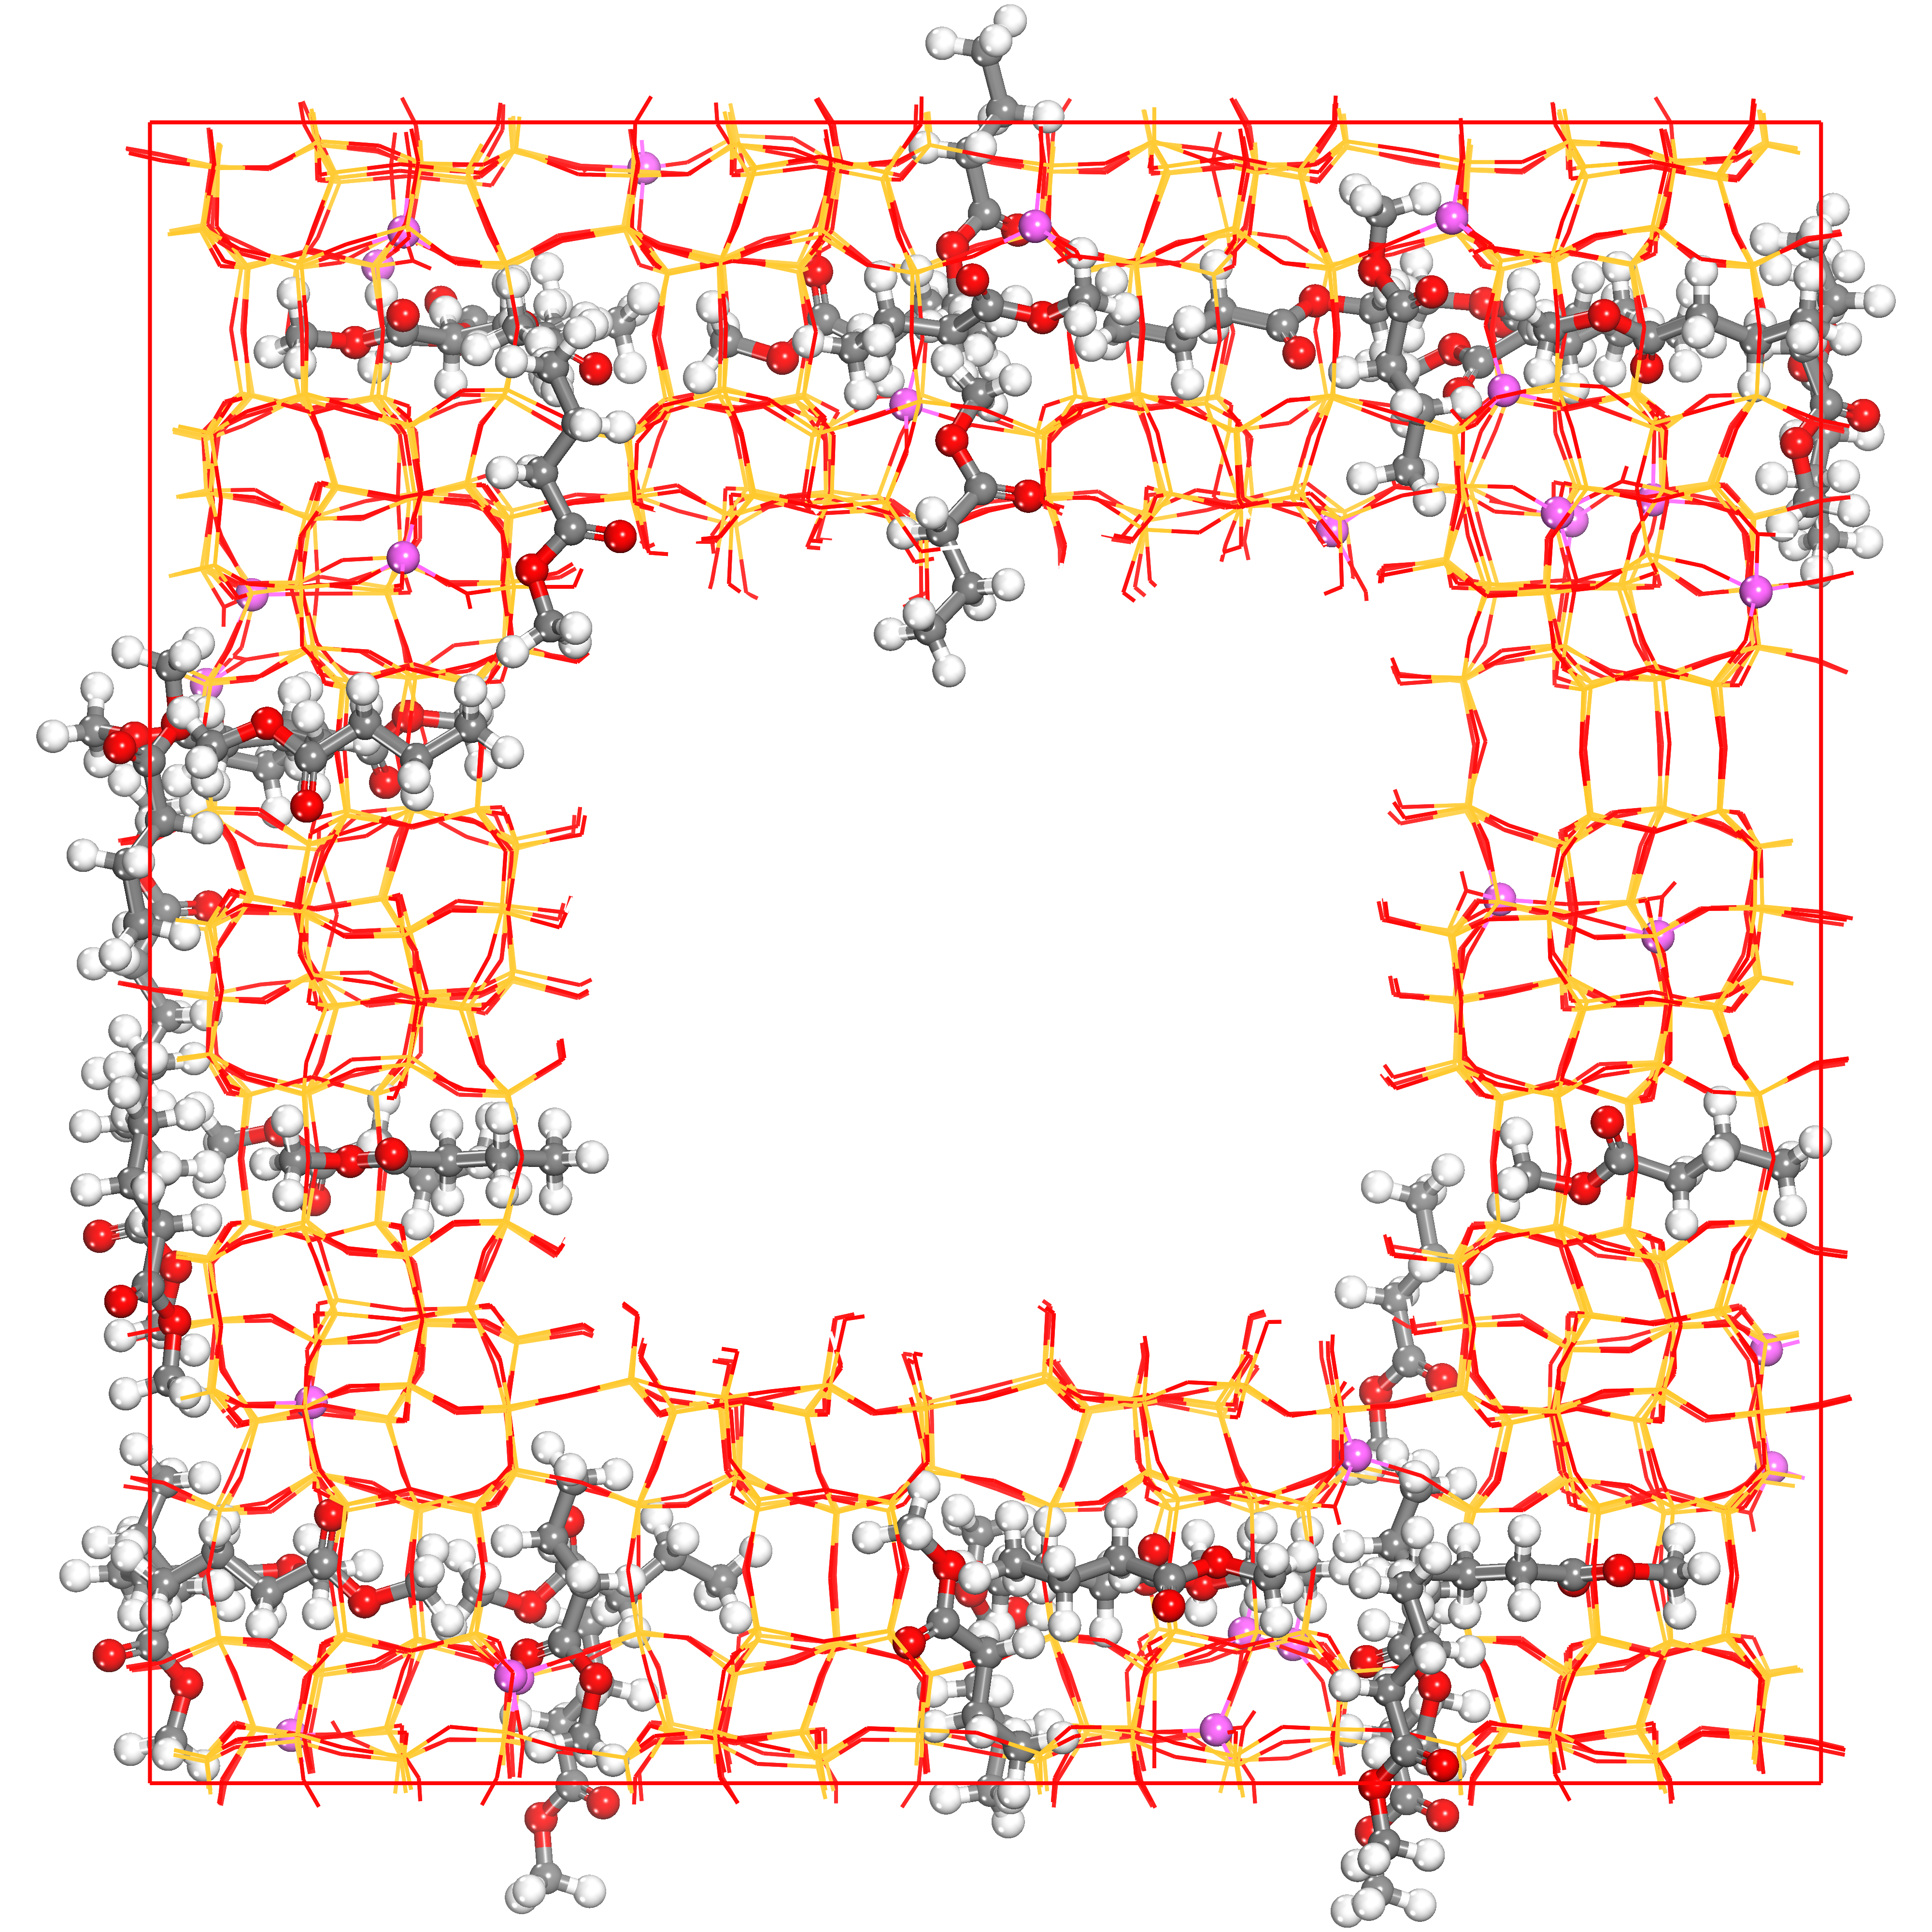
\includegraphics[width=1.8in]{figure/Diffusion/2M20.png}
    %\caption{fig2}
    \end{minipage}%
    }%
    \subfigure[60Å介孔]{
    \begin{minipage}[t]{0.3333\linewidth}
    \centering
    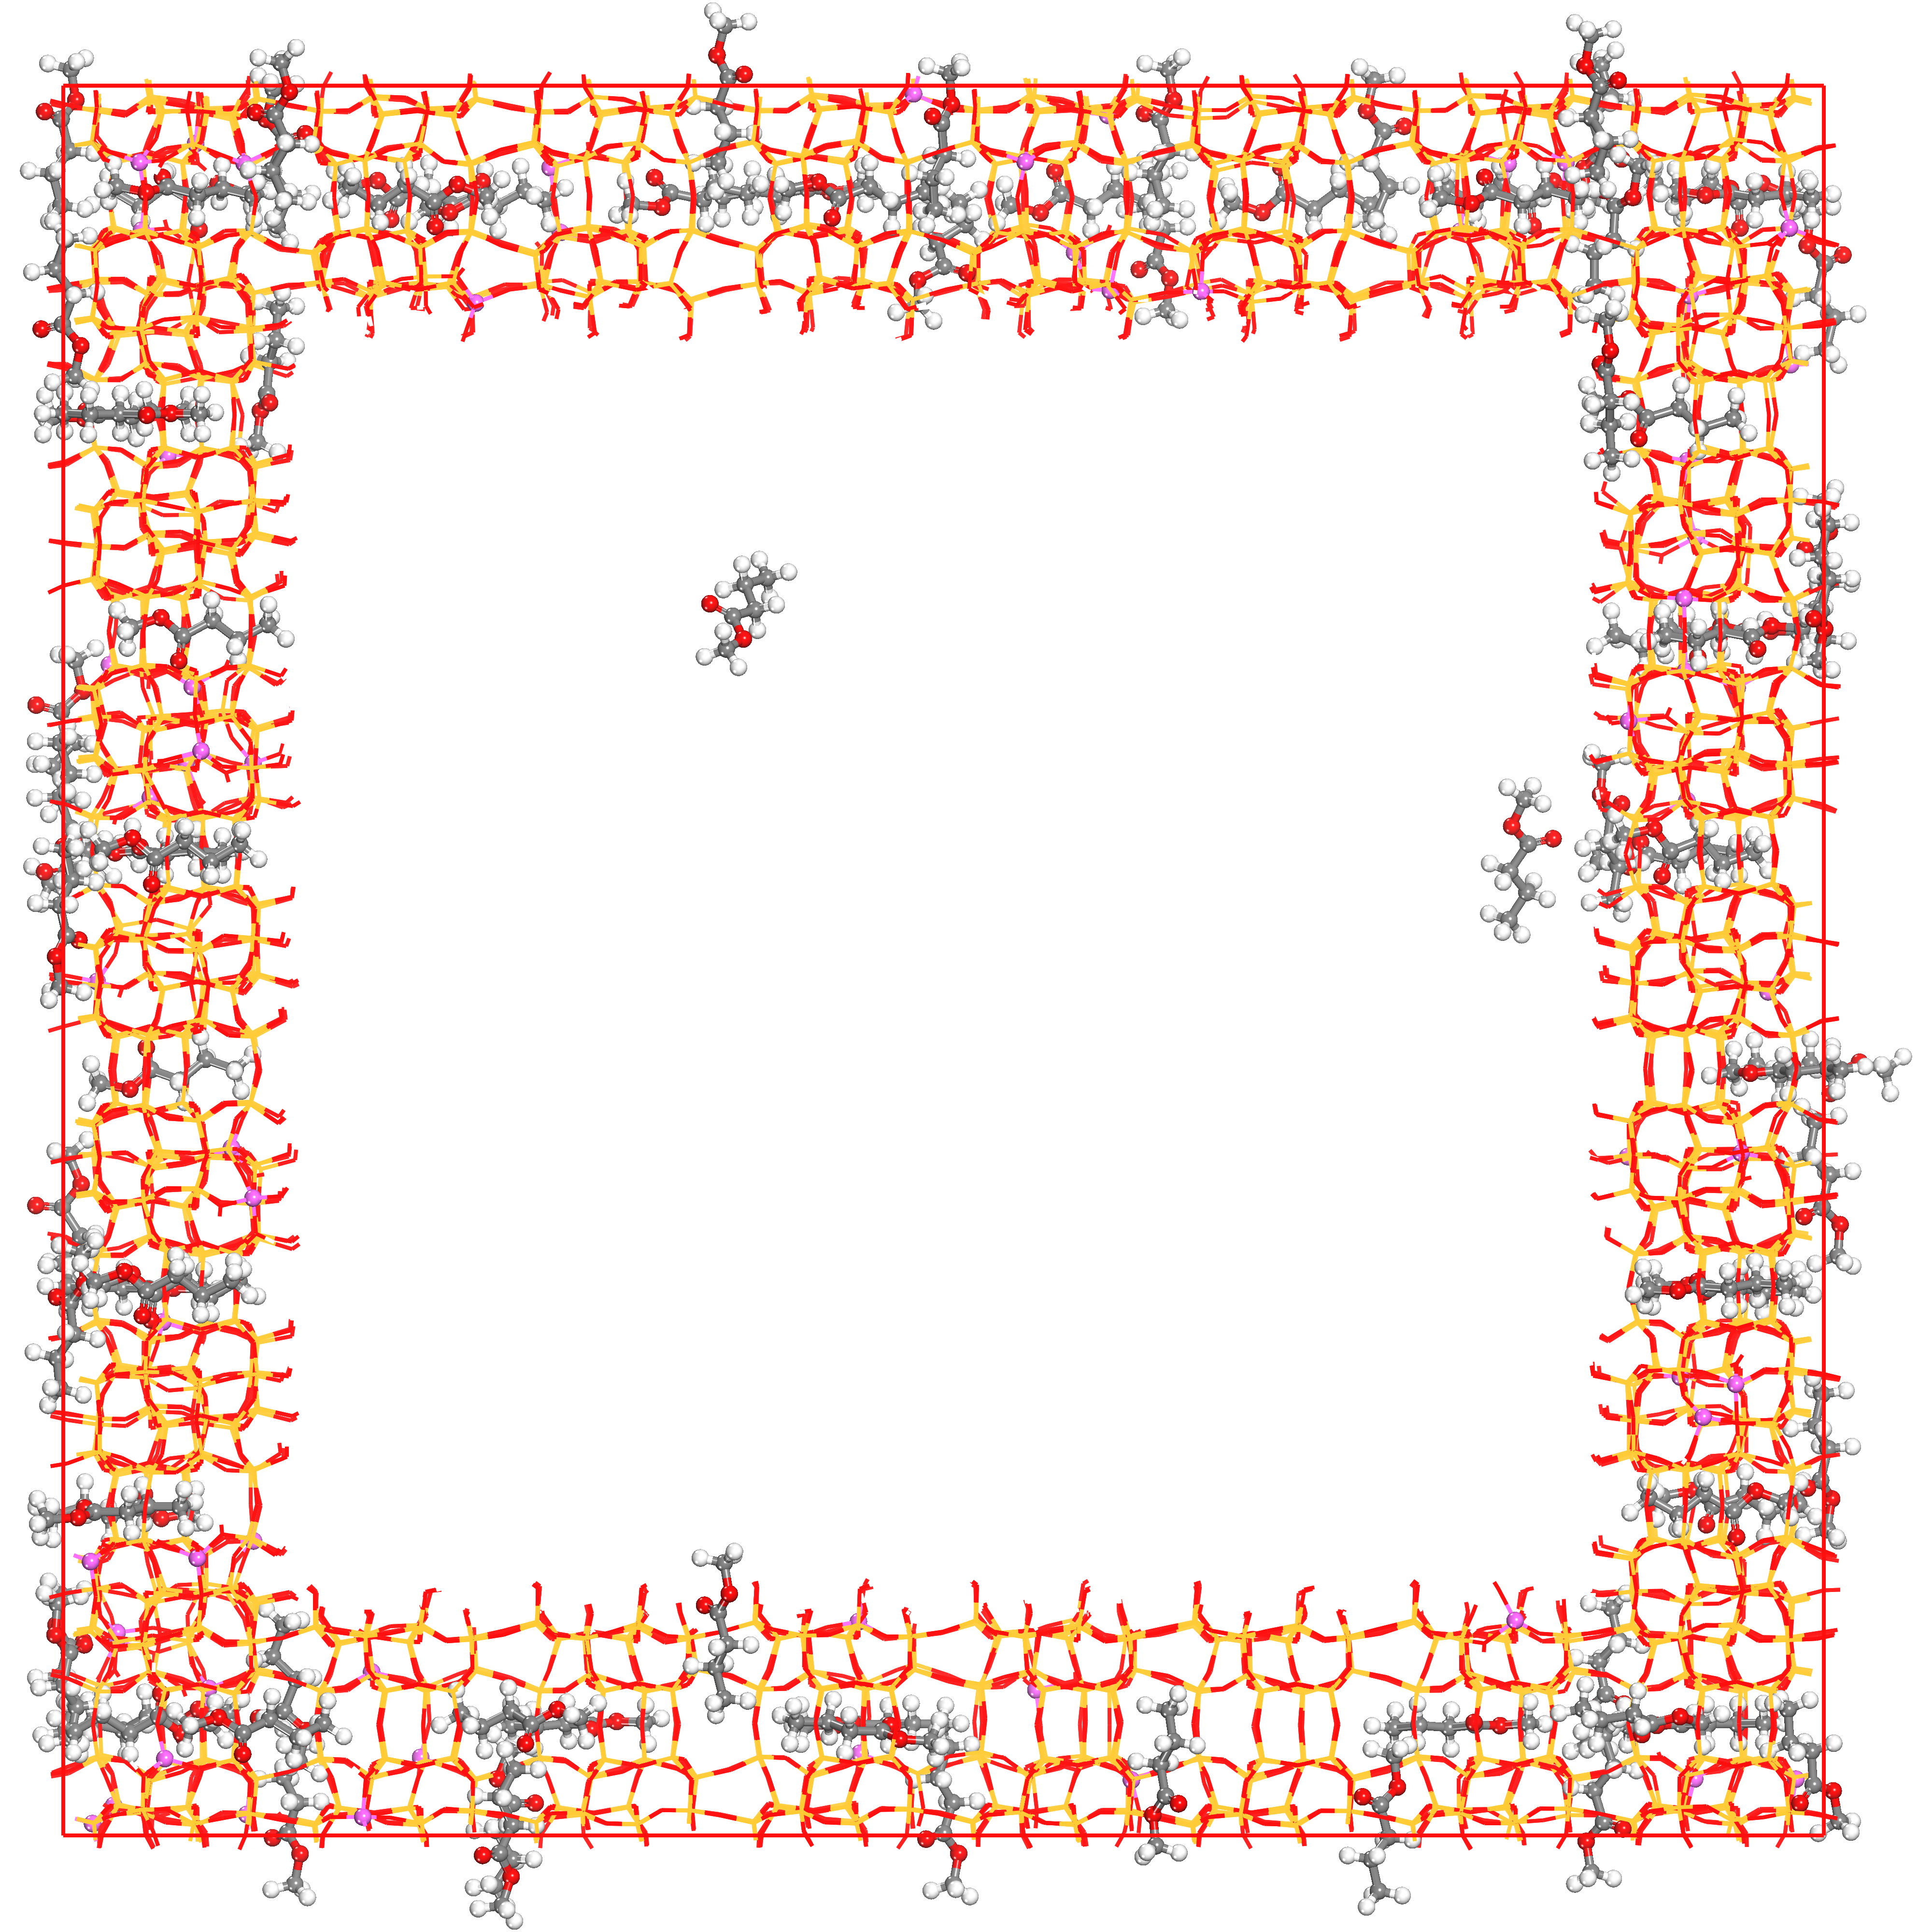
\includegraphics[width=1.8in]{figure/Diffusion/2M60.png}
    %\caption{fig2}
    \end{minipage}%
    }%
    \caption{丁酸甲酯在微孔内的初始位置示意图}
    \label{fig:MMe}
\end{figure}
\par{然后分别对各个体系进行动力学计算,温度选取为673K,模拟总时间位200ps,结果如\reffig{fig:MSDq}所示。丁酸甲酯无论是在20Å介孔的微孔内,还是在60Å介孔的微孔内,它的均方位移随时间变化的曲线的斜率几乎和在微孔分子筛内的一样大,具体的拟合结果如\reftab{tab:MMa}所示。}
\par{由\reftab{tab:MMa}可知,在20Å介孔和60Å介孔中的扩散系数几乎一样大,只比在微孔中的扩散系数大9.4\%,这说明在丁酸甲酯进入微孔后的前200ps内,丁酸甲酯几乎没有从微孔进入介孔,而是在微孔内做着受限运动,这与从扩散轨迹得到的结论是一致的。但因为介孔中的活性吸附位和一般吸附位都临近介孔,所以丁酸甲酯受到的空间位阻与在微孔中的相对较小,所以扩散系数依然比在微孔中的大,这与温度对在微孔中的等量吸附热的影响比在介孔中的小的解释是一致的。}

\begin{figure}[H]
    \centering
        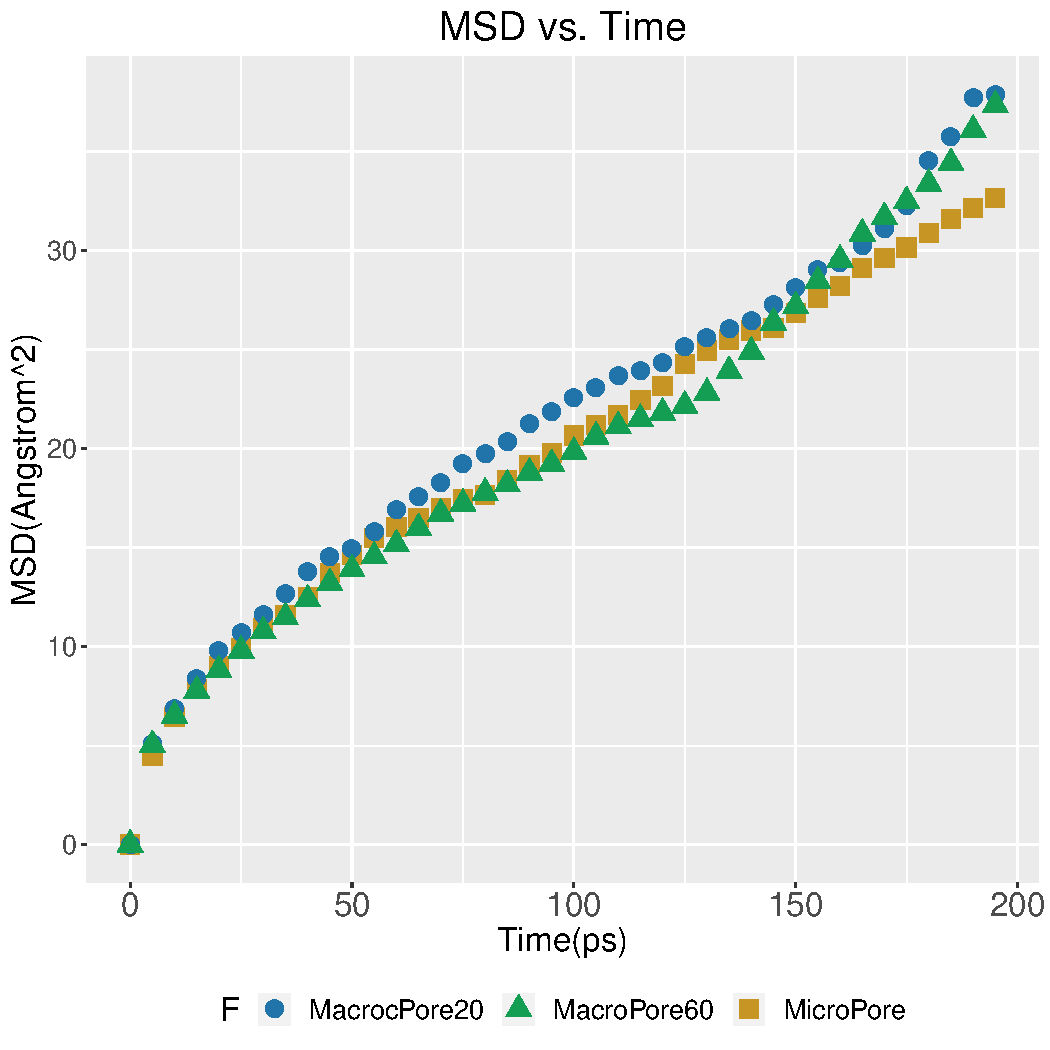
\includegraphics[width=0.5\textwidth]{figure/Diffusion/MSD.pdf}
    \caption{丁酸甲酯在不同孔径H-ZSM-5分子筛的微孔内的MSD vs. Time图}
    \label{fig:MSDq}
\end{figure}

\begin{table}[H]
	\small
	\centering
	\caption{丁酸甲酯在不同分子筛微孔中的扩散系数对比表}
	\begin{tabular}{p{2.5cm}<{\centering}p{3cm}<{\centering}p{3cm}<{\centering}P{2.2}}
        \toprule
        孔径&\makecell{MSD曲线斜率\\(Å$^2$/ps)}&R$^2$&\multicolumn{1}{p{3cm}<{\centering}}{\makecell{扩散系数\\(×$10^{-10}$m$^2$/s)}}\\
        \midrule
        微孔&0.1413&0.9773&23.55\\
        20Å介孔&0.1546&0.9729&25.77\\
        60Å介孔&0.1545&0.9777&25.75\\
		\bottomrule
	\end{tabular}
	\label{tab:MMa}
\end{table}




\subsection{本章小结}
\par{本章在673k(催化裂化温度)和100kPa(常压)下对丁酸甲酯分子在微介孔H-ZSM-5分子筛上的扩散进行了模拟,分析得到了丁酸甲酯的均方位移随时间的变化曲线,并根据斯托克斯 - 爱因斯坦方程计算得到在微孔、20Å介孔和60Å介孔分子筛中的扩散系数,得到了以下结论:}
\begin{enumerate}
    \item 丁酸甲酯扩散系数的大小顺序为60Å介孔> 20Å介孔$\gg$微孔,这个结果与实验结果一致\cite{christensen2003catalytic,meunier2012influence}。介孔 H-ZSM-5 分子筛相对于传统的微孔 H-ZSM-5 分子筛,具有着更高效的质量传递性质。但随着孔径的增大,孔径大小对扩散系数的影响变小:从微孔到20Å介孔,扩散系数增加了89.6倍;而从20Å介孔到60Å介孔,扩散系数只增加了1.4倍。
    \item 丁酸甲酯要从介孔进入微孔,取向和孔径方向必须一致,否者将会被分子筛弹开,这说明H-ZSM-5分子筛具有很高的择形性。
    \item 当丁酸甲酯进入微孔后,在介孔分子筛中的微孔的扩散系数只比在微孔中的大9.4\%,说明丁酸甲酯几乎不能再从微孔进入介孔。
\end{enumerate}
